\PassOptionsToPackage{dvipsnames}{xcolor}
\documentclass[a4paper,11pt]{book}
\usepackage[]{geometry}

\usepackage{ucs}
\usepackage[utf8]{inputenc}
\usepackage{amsmath}
\usepackage{amssymb}
\usepackage{siunitx}
\usepackage{cancel}
\usepackage[italian]{babel}
\usepackage{fontenc}
\usepackage{graphicx}
\graphicspath{{img/}}
\usepackage{circuitikz}
\ctikzset{
    resistors/scale=0.7,
    capacitors/scale=0.7,
    inductors/scale=0.7,
    sources/scale=0.7
    }

\usepackage{float}
\usepackage{xcolor}

\usepackage{hyperref}
\hypersetup{
    colorlinks=true,
    linkcolor=black,
}
\usepackage{arydshln} % dashed lines in matrix (array)



%Definizione 'globale' larghezza immagini
\newcommand{\picwid}{0.35\linewidth}
\usepackage{tikz}
\usepackage{pgfplots} % Plot dei grafici
\pgfplotsset{compat = 1.18}
% Riduzione tempi di compilazione esternalizzando le figure in pdf separati
\usepgfplotslibrary{external}
%\usetikzlibrary{pgfplots.external}
\tikzexternalize[prefix=tikz/]
\usetikzlibrary{patterns} % libreria per disegnare i pattern
%\tikzset{prefix={tikz/}}
\usepackage{pstricks-add}

\usepackage{caption}
\usepackage{subcaption}

\usepackage{polynom}

\newcommand{\Lap}{\ensuremath{\mathcal{L}}} %L di Laplace
\renewcommand{\Re}{\ensuremath{\mathfrak{Re}}} %Parte reale
\renewcommand{\Im}{\ensuremath{\mathfrak{Im}}} %Parte immaginaria

\newcommand{\infint}{\ensuremath{\int_{-\infty}^{+\infty}}} %Integrale da -inf
%a +inf
\newcommand{\kinfsum}{\ensuremath{\sum_{k=-\infty}^{+\infty}}}
\newcommand{\ninfsum}{\ensuremath{\sum_{n=-\infty}^{+\infty}}}

\newcommand{\sinc}{\ensuremath{\text{sinc}}}

\usepackage{diagbox} %pacchetto linea diagonale per tabelle
\usepackage{booktabs} % toprule midrule e bottomrule
\usepackage{steinmetz} %pacchetto per notazione angolo

\usepackage{bodegraph} %pacchetto per diagrammi di Bode

\date{\today}
\title{Appunti Sistemi Automatici di Misura}
\author{Daniele Olivieri}
\begin{document}
\maketitle
\tableofcontents
\chapter{Introduzione ai sistemi automatici di misura}
Nel seguente esempio si riporta come viene effettuato il collaudo di un filtro
passa-basso, si organizza il comparto di misura disponendo un generatore di
segnale opportunamente configurato, il DUT (Device Under Test) e uno strumento
di misura.

Per effettuare il collaudo del filtro va organizzato il banco di misura
prendendo un generatore di
segnale (sorgente)
applicando uno stimolo di tipo sinusoidale e usando successivamente un
oscilloscopio o un multimetro
per misurare la grandezza
in ingresso e quella in uscita.

Effettuando la misura dei due valori e calcolato il guadagno è poi possibile
riportare i valori su
un grafico e realizzare la maschera del filtro, la prova va effettuata con più
valori di frequenza.

Considerando una n-pla di frequenze con n sufficientemente grande si può
ripetere il test
rispettando una ovvia semantica, configurando prima la sorgente, attendendo un
tempo di
assestamento, poi effettuando le misure con il sistema a regime stabile.

Il tecnico coordina l'attività degli strumenti attivando la sorgente al tempo
giusto e attiva
l'intervento del multimetro quando è necessario l'intervento del multimetro,
eseguendo il test in
maniera ordinata da frequenze più basse a più alte o viceversa, sarebbe invece
curiosa una scelta
disordinata delle frequenze, nonostante talvolta abbia senso farlo, ad esempio
su dispositivi con
comportamento "isteretico".

\begin{figure}[h]
\centering
\begin{circuitikz}[]
\draw
 (0,0) to [short , *-] ++(1,0)
        to [R,l=R] ++(2,0)
        to [C,l=C] ++(0,-2) to [short,-*] ++(-3,0);
\draw (0,-2) to [open,v^>=$v_{in}$] ++(0,2);
\draw (3,-2) to [short,*-*] ++(1,0)
             to [open,v=$v_{out}$] ++(0,2)
             to [short, *-*] ++(-1,0);
\end{circuitikz}
\caption{Filtro passa-basso}
\end{figure}

Nell'analisi di un filtro è anche importante studiarne la \textit{fase},
potrebbe essere
presente anche una maschera della risposta in fase richiesta dal committente,
ovvero lo sfasamento
prodotto dal DUT alle basse frequenze; si ritiene che le deviazioni siano
contenute se i punti vicini in
frequenza sono vicini tra loro in fase.

Per misurare lo sfasamento tra segnali isofrequenziali, è possibile usare
un oscilloscopio
oppure strumenti dedicati come i contatori universali, utilizzando il contatore
"counter" a due
canali si può misurare il ritardo di fase dell'uscita rispetto all'ingresso.
%AGGIUNGI IMMAGINE SFAASAMENTO
\begin{figure}[h]
\centering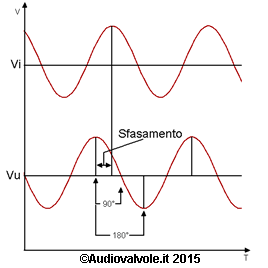
\includegraphics[width=0.4\linewidth,trim={0 4mm 0
0},clip]{misurasfasamento}
\caption{$\Delta\varphi = 2\pi \frac{\tau}{T_0}$}
\end{figure}


\subsection{Ruolo dell'operatore}
Questo ruolo può essere demandato per realizzare il processo in modo automatico,
in questo caso l'operatore
svolge il processo di coordinamento tra le sorgenti, analizzando i risultati dei
vari strumenti per
elaborare i risultati e annotarli in un diagramma.

Queste azioni possono essere demandate ad un'unità funzionale (UF) che svolge il
lavoro
dell'operatore, quest'unità è spesso un calcolatore, si possono attivare infatti
le funzioni degli
strumenti colloquiando attraverso questi tramite un'opportuna interfaccia
digitale, ovvero uno
strumento elettronico-digitale può essere configurato senza alcuna azione fisica
sul suo front
panel ma può essere configurato tramite la sua interfaccia, ovvero inviando allo
strumento una
sequenza di caratteri, una stringa, che viene decodificata e interpretata
dall'interfaccia dello
strumento, ad esempio:

Stringa per generare una forma d'onda sinusoidale di 10 V picco-picco, 1000 Hz
e un offset DC di 0 V:

\noindent
\verb|APPLY:SINusoidal 10, 1000, 0|

Quest'operazione si poteva fare a partire dagli anni 70, si realizzarono dunque
le prime stazioni
automatiche di misura.
L'unità funzionale è una macchina che può essere programmata, solitamente un PC,
era collegata ai
vari strumenti attraverso un BUS, deve poter inviare e ricevere messaggi e
informazioni ai vari
strumenti di misura.

Le spinte per cui si andò a studiare e applicare soluzioni di questo genere
erano legate ad
esigenze di incrementare l'affidabilità e velocizzare i processi di misura e
ridurne i costi.

Il collaudo affidato ad un tecnico richiede un certo tempo (del tecnico), se si
effettua produzione
di massa di dispositivi questa operazione manuale è impensabile, si effettua
inizialmente un
collaudo campionario, non si collauda ogni singolo campione ma deve comunque
essere una popolazione
rappresentativa, se anche si producono un milione di pezzi almeno un centinaio
andrà
collaudato, quanto tempo ci vorrebbe con un operatore umano? I tempi sarebbero
troppo lunghi,
l'affidabilità del collaudo è inoltre scarsa essendo affidata a all'operatore
umano, nella prima
ora ad esempio il tecnico lavora bene, nelle successive sarà sempre più stanco
\textit{lanciando i filtri
passa-basso dalla finestra}, il costo umano per le risorse umane inoltre è
elevato.

Se si programma un PC con tutte le istruzioni, la configurazione dello
strumento di misura, oscilloscopio a due canali, sarà del tipo

\begin{verbatim}
MEAS:CH1:VAC?
MEAS:CH2:VAC?
\end{verbatim}

queste istruzioni possono essere inserite in una struttura ciclica per ogni
valore di frequenza. Ne guadagno in affidabilità, un macchina programmata
quando esegue una struttura ciclica, non si stanca nella riproduzione
ripetitiva delle stesse azioni, la macchina non fa altro di ciò che è
codificato nelle istruzioni.
Se ne guadagna anche nel tempo di interazione per
configurare la sorgente ad esempio che va a regime in tempi inferiori a quelli
necessari all'operatore a cambiare le impostazioni, invece mediante
l'interfaccia le istruzioni e le risposte ottenute hanno ordini di grandezza di
gran lunga inferiori, lo stesso intero collaudo sulle varie frequenze può essere
eseguito in frazioni di secondi.

Di contro il controller non è in grado di interagire in caso di eventi
imprevisti se questi non
sono appunto "previsti" e configurate le rispettive risposte dell'unità di
controllo.
L'operatore dovrebbe trasferire tutta la sua conoscenza nella macchina,
aggiungendo inoltre
ulteriori sensori alla stazione di misura, magari non direttamente collegati al
fenomeno.

Sostenuto l'investimento iniziale della programmazione dell' UF non è più
necessaria una squadra di
tecnici al fine di collaudare tutti i DUT, è necessario solo un tecnico (o una
macchina) che
posizioni e selezioni gli oggetti che superano il test o meno.

\section{Interfaccia standard IEEE 488 - GPIB}
La seguente interfaccia è ritenuta uno standard dagli anni 70, GPIB sta per
\textit{General Purpose Interface Bus} sviluppata da HP, successivamente il
ramo riferito agli strumenti di misura è diventato Agilent e poi KeySight.

Inizialmente l'interfaccia si chiamava HPIB, gli altri costruttori poi
standardizzarono le specifiche dell'interfaccia per complementare i loro
strumenti di misura con quest'interfaccia, presentano un certo connettore con
una porta standard.
\begin{figure}[h]
\centering
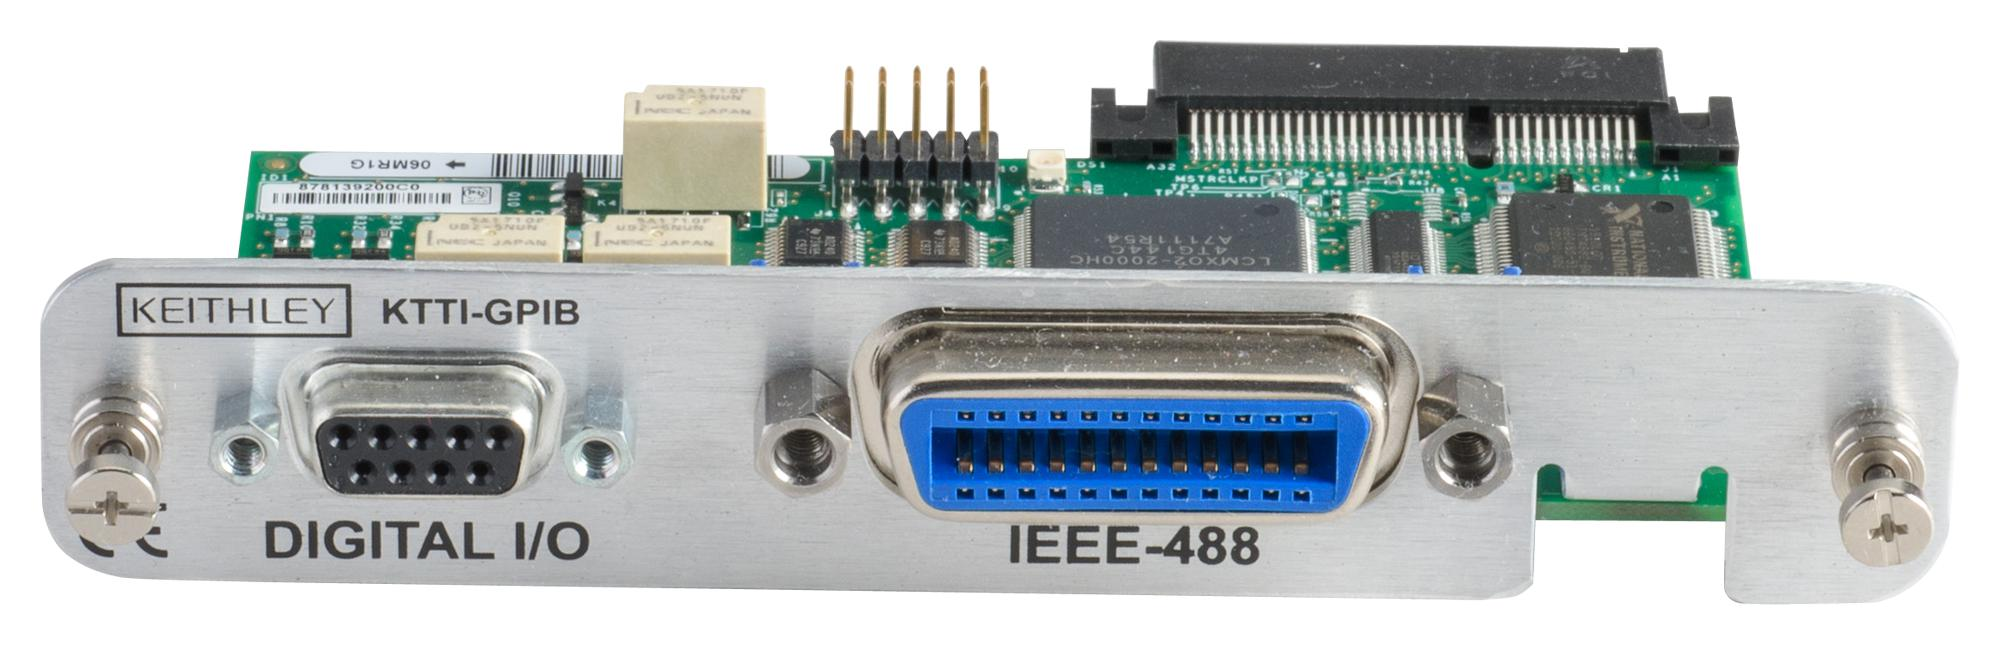
\includegraphics[width=0.9\linewidth]{GPIB}
\caption{Periferica GPIB con rispettiva porta (in blu)}
\end{figure}

Il PC potrebbe non essere disposto dell'interfaccia GPIB, si potrebbe
aggiungere una scheda PCI per avere le funzionalità della porta GPIB, oggi si
preferisce utilizzare delle versioni miniaturizzate GPIB-USB rendendo il
collegamento dell'interfaccia più semplice.

Per realizzare il collegamento si utilizza un connettore standard della
lunghezza solita di 2 m con dei connettori ``ermafroditi'' rendendo possibile
impilare i connettori nello stesso punto.

La topologia del BUS non è classificabile né di tipo a ``stella'' con un nodo
principale, né c'è un BUS ad anello chiuso (daisy chain), si possono realizzare
topologie ibride per raggiungere ed interconnettere tutte le unità tra loro, il
BUS contiene 25 linee, ogni linea verrà forzata ad un certo potenziale
elettrico, questo verrà condiviso tra tutti i dispositivi collegati al BUS, a
causa del collegamento elettrico franco, il potenziale sarà lo stesso.

Lo standard fornisce le specifiche elettriche, meccaniche e funzionali.
Le linee attive all'interno del BUS sono in realtà 24, la venticinquesima è
inutilizzata, sono tutte linee binarie, ossia possono trasferire
due tipi di informazioni 0 o 1 come un bit se il livello di tensione è alto o
basso, gran parte delle linee sono gestite in logica negata, se la tensione è
alta il bit è 0 e viceversa livello di tensione basso il bit è 0.

Le specifiche elettriche affermano che per leggere 0 la tensione deve essere
superiore a 2V, per leggere alto 1 la tensione deve essere inferiore a 0.8V.

Specifiche funzionali, le linee sono adibite ad implementare delle funzioni.
\begin{itemize}
\item 5 sono dette di GIM \textit{General Interface Management}
\item 3 sono usate per la sincronizzazione, implementano il protocollo di
handshake
\item 8 per la trasmissione di dati DIO
\item 8 di riferimento, solitamente messe a massa
\end{itemize}

Le linee GIM codificano comandi universali monolinea, ogni linea ha il suo
comando, vengono riferite con degli acronimi:
\begin{itemize}
\item IFC interface clear, per eseguire il reset dell'interfaccia
\item REN Remote enable, abilita il funzionamento remoto, necessaria al
controller ad informare gli strumenti che saranno controllati da remoto e non
dal loro pannello, si può evenualmente disabilitare completamente il pannello
rendnedolo ``sordo'' a malintenzionati che potrebbero alterare il processo di
misura
\item ATN attention, distingue due regimi di funzionamento, il regime ``command
mode'' dal regime ``device mode''
\item SRQ richiesta di servizio ``service request''
\item EOI End of Identify, ha una duplice funzione a seconda del regime in cui
ci si trova
\end{itemize}

\subsection{Come avviene la misura automatica}
Si considera una stazione di misura, si immagina che il controller sia un PC che
effettui il collaudo del filtro passa-basso,
innanzitutto attesta (\textit{attesta ovvero porta a massa?}) la linea IFC
portandola da 0 a 1, resettando tutte le interfacce, successivamente la linea
REN (controllo remoto) passa da 0 a 1. Poi si attesta la ATN, si passa in
regime di command mode,
in questo regime il controller esercita l'azione di coordinamento assegnando ai
vari strumenti di misura dei ruoli e i ruoli possibili sono: \textit{TALKER} o
\textit{LISTENER} ovvero lo strumento che invia dati al controller o riceve
dati dal controller o da un altro talker, due ulteriori ruoli sono
\textit{CONTROLLER} (non assegnabile a tutti gli strumenti), può essere comodo
avere più controller; il quarto ruolo è ``ozioso'' \textit{IDLE}, non
effettuano alcuna azione, non vengono coinvolti nella fase di misura.

\verb|IFC>REN>ATN|

Per assegnare un ruolo a ciascuno strumento, il controller utilizza gli
indirizzi, dei numeri identificativi associati univocamente e staticamente agli
strumenti, si hanno a disposizione 31 indirizzi primari, da 0 a 30, l'indirizzo
0 è riservato al controller di sistema, non utilizzabile. È possibile che ci
siano altri controller.

Il controller invia al BUS dei comandi di configurazione, di interfaccia e
tutti i dispositivi devono essere liberi sul BUS.
Se il controller vuole assegnare al generatore, identificato ad esempio con 1,
configura
le linee dati e invia l'informazione nel byte dati, nei 5 bit meno
significativi inserisce l'indirizzo dello strumento a cui vuole assegnare il
ruolo.
Il sesto e il settimo bit (capability code) assegnano i due ruoli di
\textit{listener} (01) e \textit{talker}(10). Va sempre garantita la parità del
byte come controllo degli errori di trasmissione, il numero di ``1'' nel byte
dati deve sempre
essere pari, ad esempio per impostare il generatore con indirizzo 1 a listener
(01), invia il seguente byte

\verb|00100001 (!)|

il bit più significativo viene impostato a 0 o 1 per mantenere la parità.

Il controller
informa a tutte le unità il ruolo di parlatore a sè stesso, nel campo
indirizzo di 5 bit inserisce l'indirizzo 0, nel sesto il codice che identifica
il parlatore (10), si avrà dunque il seguente byte:

\verb|11000000 (@)|

Nei byte sono associati i rispettivi codici \verb|ASCII|, rilasciando la linea
ATN, ovvero tornando alta (0), si ritorna in regime di funzionamento di
\textit{device
mode}, le unità che non sono state chiamate in alcun ruolo si pongono in stato
IDLE e non prestano attenzione a ciò che viaggia sul BUS, partecipano alla
comunicazione, in questo caso solo la sorgente e il controller.
In command mode invece i messaggi vengono letti da tutti i dispositivi.

Il comando in formato ASCII viene inviato un carattere alla volta, la sequenza
di byte viene trasferita sui canali DIO dal parlatore e recepiti
dall'ascoltatore, i tempi di trasmissione sono solitamente di una manciata di
secondi.

Nel regime di Command Mode viaggiano i comandi di interfaccia standard,
rilasciata la linea la comunicazione avviene con il linguaggio di dispositivo,
ogni dispositivo può avere il suo linguaggio.


\section{Approfondimenti sul BUS IEEE 488 - GPIB}
Presenta 5 linee di GIM tra le quali
\begin{itemize}
 \item IFC
 \item REN
 \item ATN
 \item SRQ
 \item EOI
\end{itemize}
tre linee per la sincronizzazione che seguono il protocollo ``handshake'',
8 linnee per la trasmissione dati e 8 linee di riferimento (GND).

Un esempio di processo di misura da automatizzare è ancora il collaudo di un
doppio bipolo che realizza un filtro passa basso, il banco è costituito da tre
strumenti e un controller.
Il controller è un PC con interfaccia IEEE488, un counter a due canali, una
sorgente a singolo canale e un multimetro digitale a due canali.
Anche gli strumenti, come il PC sono dotati di interfaccia.

Il counter serve a misurare lo sfasamento tra i segnali isofrequenziali, il
multimetro misura il guadagno introdotto dal filtro, solitamente un guadagno
unitario nella banda passante che si riduce man mano entrando nella frequenza
di transizione, oltre la frequenza di taglio.

Il controller attesta la linea IFC e subito dopo da un secondo comando
universale unilinea REN in cui specifica alle unià periferiche che riceveranno
i comandi tramite interfaccia e non tramite pannello. Si attesta poi la linea
ATN e la stazione di misura viene posta in regime ``command mode''.

Il controller in questo funzionamento assegna dei ruoli agli strumenti mediante
un meccanismo di indirizzamento, ad ogni strumento sarà assegnato un indirizzo,
un intero che va da 1 a 30, per specificare quest'indirizzo si utilizzano 5 bit.

Con 5 bit si realizzerebbero $2^5$ combinazioni ma l'indirizzo 0 è riservato al
controller mentre l'indirizzo 31 è necessario all'abilitazione di un indirizzo
secondario, come ad esempio un modulo particolare di un certo strumento.

Sono comunque poche le applicazioni che necessitano del meccanismo di
indirizzamento secondario.

Si assegni alla sorgente l'indirizzo 1, al multimetro l'indirizzo 2 e al
counter l'indirizzo 8.
Per configurare inizialmente la sorgente va inviato un comando in regime
``device mode'' comprensibile solo alla sorgente, dopo averle assegnato un
ruolo, si riserva il bus ad una comunicazione dedicata tra un talker e un
listener.

Per assegnare il ruolo di listener alla sorgente si utilizzano lel linee dati
usando i 5 bit meno significativi l'indirizzo dello strumento, assegnando un
ruolo mediante il sesto e il settimo bit, l'ottavo bit rispetta la regola della
parità.

Il controller assegna il ruolo di listener al dispositivo con indirizzo 1

\verb|00100001 - A - !|

Si configura il controller come listener

\verb|11000000 - \@ - MTA0|

Si rilascia infine la linea attention (ATN) passando al regime device mode, il
counter e il multimetro non hanno visto il loro indirizzo, restando in idle.

La comunicazione sul BUS prevede sempre un solo talker ma può avere più
listener a patto che comprendano lo stesso linguaggio.

Gli strumenti di misura hanno sempre in allegato dei manuali, o una
documentazione con una sezione riservata alla programmazione dello strumento.

Un comando che solitamente si usa per configurare la sorgente è il comando

\verb|APPLy:SINusoidal 10,1000,0|

Nella sintassi estesa si può aggiungere l'unità di misura dei valori.
La sintassi contratta è composta solo dalle parti in maiuscolo, la sintassi è
decisa dal costruttore.
Si potrebbe in teoria assegnare un comando per ciascun carattere, riducendo il
numero di caratteri da inviare.

La velocità di throughput può raggiungere velocità pari al megabyte/s.
Lo standard richiede di non utilizzare cavi di lunghezza maggiori.

Rendere il linguaggio dello strumento stringato si è riscontrato che i comandi
per attivare le funzioni sono più semplici da memorizzare.
La scelta dei costruttori è stata quella di configurare i comandi da renderli
facilmente memorizzabili.

Durante la configurazione, la sorgente inizia a a generare il segnale stabile,
rendendo l'interfaccia indipendente.

All'invio di ogni byte in device mode, si attiva una procedura di
configurazione per lo scambio dei dati con conseguente sincronizzazione

Se lo strumento riceve un comando errato, va in errore.

Il talker configura le linee dati utilizzando la procedura di handshake per
sincronizzare la comunicazione, quando ha terminato il messaggio, invia l'EOI,
End Of Identify

Terminata la comunicazione dal sistema sorgente, a talker torna il possesso del
bus.

In regime command mode il controller associa il ruolo di listener
all'indirizzo 2

\verb|00100010|

e ancora il ruolo di listener a sé stesso, vanno ora inviati dei comandi di
\textit{deselezione} degli strumenti precedentemente attivati, ad esempio si
invia il seguente comando per deselezionare i listener precedentemente attivati

\verb|00111111 - ?|

oppure per deselezionare i talker con il carattere ``\_''

\verb|01011111 - _|

Per ottenere il risultato dal multimetro dopo averlo impostato come listener si
invia un comando di QUERY, terminato da punto interrogativo (?)

\verb|MEAS:CH1:VAC?|

Lo strumento deve conservare il risultato perché dopo una QUERY allo strumento
verrà assegnato il ruolo di parlatore e invierà il risultato al listener, il
ruolo di parlatore al dispositivo 2 si invia con il carattere B, ancora una
volta il controller si imposta come listener con il carattere ``barra
spaziatrice''

\verb|01000010 - B|

\verb|10100000 - " "|

Quando il multimetro termina la comunicazione si ritorna in regime di command
mode, si ripete la procedura per rieseguire la misura sul canale 2 (\verb|CH2|).

Lo stesso processo si ripete per il counter per eseguire la misura di
sfasamento, deseleziona precedenti listener e talker, invia una QUERY al
counter dopo averlo impostato come listener, dopo si imposta come talker per
permettergli l'invio del risultato.



Quelli presentati sono comandi multi linea universali, perché utilizzano più
linee per comunicare con i dispositivi, possono essere specifici se hanno un
indirizzo specifico e si riferiscono ad un singolo dispositivo oppure possono
essere aspecifici se inviano un comando a tutti i dispositivi come la
deselezione.

Nei linguaggi di programmazione moderni tutti questi comandi sono contenuti in
librerie che eseguono lettura e scrittura di dati da e verso il BUS mediante
comandi più semplici come ``\textit{bus read}'' e ``\textit{bus write}''.

\subsection{Driver delle linee}
Per attestare o rilasciare una linea si utilizza un transistor bipolare, è un
dispositivo comandato in corrente, iniettando una corrente di base $i_B$ si ha
la conduzione, altrimenti senza alcuna corrente si pone in regione di
interdizione, nel driver si collega il transistor mediante una resistenza di
``pull-up``, la linea va in contatto elettrico con il morsetto collettore del
BJT.

Si riporta la caratteristica del transistor, una famiglia di curve in funzione
della corrente di base $I_B$
\begin{figure}[h]
\centering
\includegraphics[width=0.5\linewidth]{BJT}
\caption{Carattaristica di un BJT}
\end{figure}

Abbondando con la corrente di base si manda in saturazione il BJT e si attesta
la linea, ponendo $V_{CE} = 0$, eliminando la corrente di base invece la
$V_{CE}$ può essere piccola o grande, questo fa sì che se la linea è condivisa
tra più driver potrebbe accadere che se un transistor vuole la linea attestata
e un altro transistor la vuole rilasciata prevarrà il driver che attesta la
linea, la corrente nel transistor in saturazione aumenta, provenendo anche
dall'alimentazione del driver interdetto; per questo motivo si utilizza il
potenziale basso per il valore logico 1, se c'è una sola interfaccia che vuole
attestare la linea, quella linea si attesta.
È implementata la logica wired-OR, basta almeno un valore 1 affinché tutta la
linea sia 1.

\begin{figure}[h]
\centering
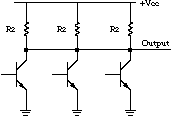
\includegraphics[width=0.5\linewidth]{wired-or}
\caption{Wired OR}
\end{figure}

Esiste un problema detto di fan-in se in un sistema con più periferiche un solo
driver assorbe correnti dagli altri driver diventerebbe troppo elevata, per
questo motivo lo standard impone un numero massimo di dispositivi pari a 15,
per non sovraccaricare il transistor in saturazione.


Non tutte le linee sono condivise, gli strumenti di misura ad esempio non
possono pilotare le linee IFC, REN e ATN riservate al controller, possono solo
osservarne lo stato ma non alterarlo.

\subsection{Sincronizzazione}
Il clock dei diversi hardware e strumenti non è standardizzato, ciascun
dispositivo avrà il suo clock, sono definiti moduli ''asincroni`` tra loro.
Sistemi con moduli sincroni sono invece solitamente ospitati su una stessa
scheda; in una stazione automatica di misura si utilizzano strumenti
stand-alone, intercambiabili e utilizzabili in situazioni diversi.
Alcuni sistemi VXI, PCI gli strumenti stanno su scheda invece e vanno collocati
in un'altra scheda, utilizzando il clock del dispositivo ''ospite``.

Affinchè la comunicazione avvenga correttamente tra moduli asincroni va gestita
la sincronizzazione, le linee utilizzate a tale scopo sono 3, riferite con i
seguenti acronimi
\begin{itemize}
 \item DAV: ''Data Valid`` oppure ''Data Available``, gestita da chi invia il
dato
 \item NRFD: Not Ready For Data gestita da chi riceve i dati, non sono pronto a
ricevere i dati
 \item NDAC: Not Data ACcepted, gestita da chi riceve i dati, non ho ricevuto i
dati
\end{itemize}

Chi deve parlare configura le linee dati DIO in un certo istante con un
carattere arbitrario da trasferire, comunica che i dati sono pronti dopo averli
configurati, dopo essersi accertato che le periferiche sono pronte per ricevere
il dato e se hanno acquisito il dato precedente.

La linea NRFD è condivisa tra più ascoltatori, di conseguenza per quanto
precedentemente esposto, quando TUTTI gli strumenti rilasciano la linea, anche
il più lento, la linea viene rilasciata; solo allora la periferica più veloce
attesta nuovamente la linea nell'attesa della ricezione dei dati. Dopo che i
dati sono stati dichiarati validi, via via che tutte le periferiche verificano
e accettano i dati, rilasciano la linea NDAC, quando anche la periferica più
lenta rilascia la linea NDAC la linea viene rilasciata, solo allora il
parlatore, che intanto osserva la linea NDAC, riconfigura la linea dati
inserendo il dato successivo, il ciclo si ripete.

\begin{figure}[h]
\centering
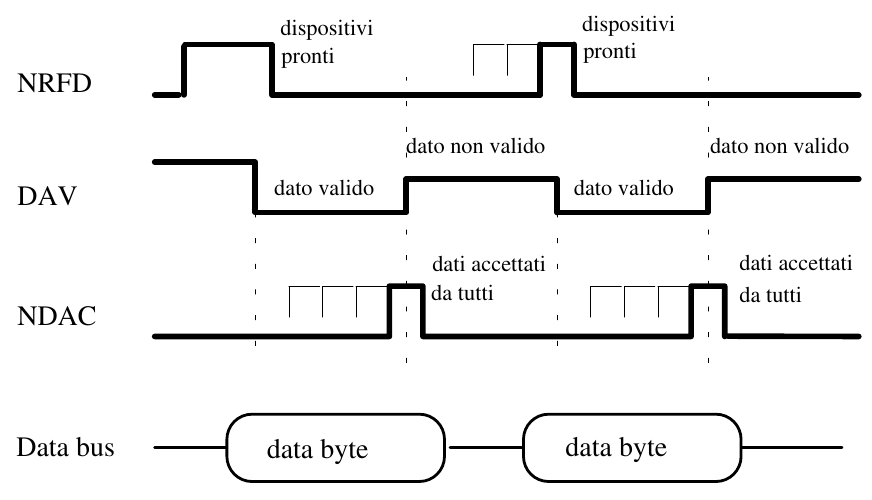
\includegraphics[width=0.7\linewidth]{sincronizzazione}
\end{figure}
Il meccanismo wired-OR permette di mantenere il dato sul BUS finché anche la
periferica più lenta non lo ha interamente acquisito, si evitano le letture
multiple alle periferiche veloci e si permette alle periferiche lente di
acquisire interamente i dati.


\subsection{Gestione delle richieste di servizio SRQ}
Quando uno strumento riceve una QUERY, mentre esegue la sua elaborazione il BUS
non resta occupato, quando ha terminato le misurazioni attesta la linea SRQ,
non si può sapere quale strumento abbia attestato la SRQ, va eseguita una
procedura di polling, di interrogazione. Esistono due tipologie di polling,
seriale e parallelo, il polling seriale consiste nell'interrogazione di tutti
gli strumenti in serie, uno alla volta.

C'è un comando multilinea universale che corrisponde al carattere ASCII SPE,
''Serial Poll Enable'' tutti gli strumenti capiscono che se sono chiamati ad
essere talker sul BUS devono trasferire sul BUS il contenuto dello status byte,
se il settimo bit è alto allora indica che quello strumento ha precedentemente
effettuato la richiesta SRQ, i restanti bit contengono l'informazione sul
motivo della richiesta.

Il polling seriale deve essere esaustivo, non posso sapere quanti strumenti
abbiano attestato la linea SRQ, terminato il polling si invia la richiesta SPD
``Serial Poll Disable'' al fine di rilasciare la linea SRQ.

La procedura di polling parallelo invece è più efficiente anche se richiede una
procedura di configurazione iniziale più onerosa, si dà un comando detto PPC
``Parallel Poll Configure'' ovvero avvia una procedura di configurazione al
parallel poll, ad ogni strumento viene assegnata una linea dati da
attestare (sono presenti 8 linee dati), una volta ricevuta la SRQ si può sapere
in anticipo quale strumento l'abbia richiesta leggendo quale linee dati sono
state attestate, in command mode(ATN) l'attestazione della linea EOI invia una
richiesta di identificazione, se la periferica aveva effettuato una richiesta
di servizio agisce direttamente sulla linea dati ponendo alto il bit che le era
stato assegnato.

Se il numero di dispositivi è maggiore di 8 si possono assegnare più
dispositivi alla stessa linea, ripetendo la procedura di polling seriale su un
gruppo più piccolo di dispositivi.

Terminata la configurazione di parallel poll si invia il comando PPU ``Parallel
Poll Unconfigure`` per disabilitare la risposta di tutti i dispositivi al
parallel poll.


\section{Interfaccia VXI IEEE 1155}
Un'interfaccia che raccolse una certa attenzione fu la tecnologia \textbf{VXI},
si perse l'aspetto stand-alone dello strumento dato che i sistemi VXI sono molto
compatti e ospitati in un cestello, sono strumenti su scheda elettronica,
possono essere alloggiati in qualche slot, non c'è alcuno spazio negli slot per
un'interfaccia completa, si perde la caratteristica stand-alone.

Il cestello tramite il back plain alimenta le schede, l'interazione può
avvenire solo mediante l'interfaccia VXI, tramite righe di comando per
richiedere determinate funzioni.
Il vantaggio è avere una stazione di misura particolarmente compatta, la
strumentazione su scheda riesce a scambiare flussi dati tra i vari moduli ad
una velocità maggiore rispetto all'interfaccia IEEE 488.
I bus sono molto corti, a volte sono piste stampate sul back plain, c'è la
capacità di trasferire i dati in maniera efficiente.

Standard similari al VXI sono stati \textbf{PXI}, cestelli ancora più compatti,
concepiti alla stessa maniera.
Si è persa l'interfaccia degli strumenti e le unità non sono più stand-alone,
durante l'esecuzione del processo di misura non c'è alcun feedback su cosa stia
accadendo, si vedono al massimo dei LED lampeggiare, l'utilizzatore deve avere
un livello professionale più alto.
Il tecnico ha dunque un costo più alto.
In più la stessa strumentazione ha dei costi elevati, quindi non è semplice
sostituire gli strumenti più vecchi, si tende dunque a restare legati alla
soluzione, anche più vecchia, sulla quale sono stati investiti più soldi.

Gran parte delle PMI adotta infatti ancora lo standard GPIB con strumentazione
stand-alone.
Il successo è dunque stato limitato rispetto allo standard GPIB.

\section{Interfaccia I2C e SPI}
L'acronimo \textbf{$I^2C$} sta per Inter Integrated Circuit, sono protocolli di
basso livello, consentono la comunicazione tra moduli elettronici integrati,
dei chip, comparsi circa negli anni '80, comparse prima SPI sviluppata da
Motorola, la sezione che ora se ne occupa è FreeScale Semiconductor.
Il microprocessore Motorola 6800 fu molto diffuso.

Il protocollo SPI è un protocollo master-slave, saranno presenti sulla scheda
elettronica un modulo master e uno o più moduli slave.
Sono presenti più linee, le più comuni sono
\begin{itemize}
\item SLCK Linea di clock
\item MOSI Master Output Slave Input, linea uilizzata dal master
\item MISO Master Input Slave Output linea utilizzata dagli slave per
comunicare con il master
\item SS Selezione dello Slave, il master indica con quale unità vuole
colloquiare
\end{itemize}
La comunicazione è full-duplex, l'uno può parlare all'altro e viceversa
contemporaneamente, viceversa si avrebbe una comunicazione half-duplex se si
usasse una sola linea.

Per ogni comunicazione sono necessarie 4 linee che (eccetto la SS) possono
essere condivise tra i vari slave, deve invece essere necessaria una linea SS
sul chip master per ogni slave che si vuole collegare.

La linea di SLCK e SS è ad intero appannaggio del master, viceversa le altre
due linee possono essere controllate dagli slave.
Non può esistere una comunicazione diretta tra due slave.

Il protocollo non vincola la frequenza del clock, il master potrebbe decidere di
lavorare con un clock più alto op più basso, a seconda del chip disponibile.
(?) Il master si adatta allo slave facendolo lavorare alla sua frequenza
indicata.

La tipologia di comunicazioni si dividono in
\begin{itemize}
 \item Clock Polarity (0-1)
\item Clock Phase (0-1)
\end{itemize}

Il chip slave può essere impostato per configurare il dato sul fronte di
salita, e leggerlo sul fronte di discesa.
L'attività sulle linee MOSI e MISO sono sincrone.


Il Master può parlare di volta in volta con uno slave, non c'è la
possibilità di una comunicazione multipla


\section{Protocollo I2C}
Il protocollo I2C è stato utilizzato molto ad esempio per il dispositivo
Arduino.

Esistono solo due linee nel protocollo I2C, una linea di clock ed una per il
trasferimento dati, il pilotaggio delle linee avviene in maniera simile alla
linea GPIB ma si utilizzano dei mosfet al posto dei BJT.
Il protocollo è multi-master e consente di collegare tra loro non solo coppie di
dispositivi ma un insieme di \textit{n} dispositivi collegati sulla stessa
coppia.
Ogni dispositivo può diventare master sul BUS che è quindi una risorsa
condivisa.

Chi vuol parlare sul BUS dà un segnale di START che corrisponde ad un evento
anomalo, dato che lo standard prevede che la linea dati possa essere
configurata solo quando il clock è basso, la transizione della linea dati
quando il clock è alto è un evento anomalo; in generale il protocollo prevede
che la linea dati possa essere configurata solo a clock basso. Allo stesso modo
il segnale di STOP è un evento anomalo con una configurazione della linea dati
SDA con il clock SCL alto.

Ogni dispositivo presenta un indirizzo a 7bit, esiste anche un meccanismo a 10
bit, la pluralità di dispositivi è elevatissima, fino a 128 in teoria con i 7
bit, abilitando la comunicazione a 10 bit si raggiungono invece numeri enormi.

Il modulo che dà il segnale di START identifica il dispositivo slave con il
quale vuole parlare mediante il suo indirizzo, l'ottavo bit indica se il master
vuole ascoltare o leggere dallo slave, 1 voglio leggere, 0 voglio scrivere.
Dopo aver trasferito i dati (8bits) si ha il bit di risposta dell'ascoltatore
che invia il bit ACK di acknowledge, attesta la linea, la
logica non è negata quindi linea attestata è pari al livello logico 0 e
viceversa con linea rilasciata.

Si trasmettono i dati per 8 bit e chi ascolta invia un bit di ACK ogni 8 bit
ricevuti, chi parla dopo aver trasmesso il suo messaggio rilascia il BUS con
l'evento di STOP, rilasciando la linea dati quando il clock è alto.
Il bit ACK è sempre fornito da chi ascolta a prescindere se questo sia il
master o lo slave.

Nel caso in cui il master sia in ascolto questo può terminare la comunicazione
inviando un messaggio di ACK rilasciando la linea e non attestandola (bit 1)
successivamente si invia l'evento di STOP sul BUS.
Anche se il messaggio non è stato trasferito completamente, il master potrebbe
tornare in ascolto del dispositivo successivamente.

Potrebbe capitare che due unità decidano di parlare simultaneamente sulla linea
che è comunque in logica wired-or, se un dispositivo attesta la linea questa va
giù per tutti, entrambe le periferiche avviano la configurazione della linea
dati per inviare l'indirizzo della periferica slave con la quale vogliono
parlare. Se gli indirizzi sono diversi prevale allora uno dei due.

Ad esempio un master vuole parlare con lo strumento ad indirizzo 1

\verb|0000001|

mentre un altro vuole parlare con il dispositivo ad indirizzo 3

\verb|0000011|

Quando si trasmette in contemporanea il sesto bit il dispositivo che voleva
comunicare con quello ad indirizzo 3 si rende conto che non può rilasciare la
linea che invece è stata attestata dal dispositivo che comunicava con indirizzo
1, dunque si mette in IDLE e capisce che non deve continuare la comunicazione.
Si dice dunque che il dispositivo ad indirizzo 1 ha la priorità su quello ad
indirizzo 3.

Se ancora entrambi i master volessero parlare con lo stesso dispositivo il
controllo della linea avverrebbe sulla trasmissione dei dati, uno dei due
dispositivi master si rende conto in ogni caso di dover porsi in attesa.

Nella configurazione a 10bit si inviano prima quattro 1 per inviare un comando
riservato e far capire ai dispositivi che si sta utilizzando l'indirizzamento a
10 bit, 8 in un byte e i restanti due nel byte precedente.


Il CLOCK è variabile, si può lavorare in modalità slow mood o fast mood o
ancora fast mood Plus, o ancora una modalità a 3.4Mb/s, non tutte le
periferiche supportano queste velocità, il master attiva la comunicazione al
valore più alto possibile (10kHz 400kHz o 1 MHz).
Esiste un meccanismo di CLOCK stretching che consente ad una periferica di
rallentare il clock. Anche la periferica richiamata dunque può intervenire
sulla linea di clock e gestirla, dunque se una periferica che lavora
nominalmente a 10kHz dovesse aver problemi e rallentare potrebbe comunque
gestire la linea di clock e raggiungere ancora il sincronismo.

Ancora oggi si utilizzano entrambe le soluzioni SPI e I2C.




\chapter{Elaborazione dei segnali}

Chi lavora con i segnali vede il segnale come un oggetto adimensionale,
trattando il concetto di \textit{potenza} ed \textit{energia} di un segnale
senza vedere effettivamente il senso e la grandezza fisica del segnale.
Esistono i segnali di tipo \textbf{deterministico} e segnali di tipo
\textbf{aleatorio}.
Se il segnale è di natura deterministica sono in grado di determinare
l'espressione del segnale, se invece è di natura aleatoria non posso
determinare in forma chiusa il suo andamento, data appunto la sua natura
stocastica, aleatoria.

Un segnale è una grandezza fisica o misurabile che evolve nel tempo, il
segnalamento sta nelle caratteristiche dell'evoluzione temporale.
Nel caso limite il segnale può essere banale ossia costante nel tempo.

Un segnale è detto di energia ed è dotato di energia se la grandezza
\begin{equation}
 \varepsilon_x = \int_{-\infty}^{+\infty} |x(t)|^2 dt < +\infty
\end{equation}
è finita, tutti i segnali transitori che decadono in un certo intervallo di
tempo sono segnali di energia.

La potenza di un segnale è definita come
\begin{equation}
 P_x = \lim_{T\to+\infty} \left(\frac{1}{T}\int_{-T/2}^{+T/2} |x(t)|^2
dt\right) < +\infty
\label{eq:potenza_segnale}
\end{equation}

Il segnale sinusoidale ad esempio non è un segnale di energia ma è un segnale
di potenza, se si valuta il valor medio su un intervallo pari ad un periodo o
multiplo di periodo, si può determinare la potenza del segnale.

In base alle definizioni l'energia si esprime ad esempio in $V^2/s$ mentre la
potenza rimarrebbe $V^2$, anche se non ci sarebbe alcuna correlazione fisica con
la potenza elettrica. Ci sarebbe corrispondenza tra potenza del segnale e
potenza elettrica se il segnale fosse proprio $v(t)\cdot i(t)$ o nel caso
semplice $|v(t)|^2/R$.

\section{I segnali periodici}
Tipicamente in ingegneria elettrica i segnali analizzati sono periodici,
possono essere più o meno distorti ma sempre riconducibili a serie di segnali
periodici.
La classe di segnali periodici si identifica come la classe di segnali che
soddisfa il vincolo
$$
x(t+kT_0) = x(t) \forall k \in \mathrm{Z}
$$
dove $T_0$ è proprio il periodo del segnale.

Se un segnale è semplice si può esprimere con una semplice funzione
sinusoidale, oppure esistono segnali di forma canonica come i segnali
triangolari o ad onda quadra, in alternativa si può rappresentare un segnale
periodico con la sua serie di Fourier
\begin{equation}
 x(t) = A_0 + \sum_{k=1}^{\infty} A_k \cos \left( 2\pi f_0 t - \phi_k \right)
\end{equation}
con $f_0= \frac{1}{T_0}$ la frequenza fondamentale, per $k$ diverso da uno
invece si hanno altre frequenze chiamate componenti armoniche perché sono un
multiplo intero della frequenza fondamentale.
Il termine $A_0$ rappresenta la componente continua, se diversa da 0 il segnale
non è alternato.

Il termine sinusoidale si può scomporre con un termine in fase ed uno in
quadratura.

\begin{equation}\begin{aligned}
 \cos(\alpha-\beta) &= \cos\alpha\cos\beta+\sin\alpha\sin\beta \\
 x(t) &= A_0 + \sum_{k=1}^{\infty} \left[ A_k\cos\phi_k\cos(2\pi k f_0 t) +
A_k\sin\phi_k\sin(2\pi k f_0t) \right] \\
x(t) &= a_0 + \sum_{k=1}^{\infty}\left[a_k\cos(2\pi k f_0) + b_k\sin(2\pi k
f_0)\right]
\end{aligned}
 \end{equation}

I due termini sono dunque in quadratura tra loro
\begin{equation*}
\begin{aligned}
\left\{\begin{aligned}
a_k &= A_k\cos\phi_k\\
b_k &= A_k\sin\phi_k
\end{aligned}\right. \\
&\text{dunque}\\
A_k &= \sqrt{a_k^2 + b_k^2}\\ \left\{
\begin{aligned}
\phi_k &= \tan^{-1}\left(\frac{b_k}{a_k}\right) \quad a_k > 0 \\
 \phi_k &=\pi - \tan^{-1} \left(\frac{b_k}{a_k}\right) \quad a_k < 0
 \end{aligned}\right.
\end{aligned}
\end{equation*}

Si ricorda la seguente definizione della formula di Eulero
\begin{equation}
 e^{\pm jx} = \cos{x} \pm j\sin{x}
\end{equation}
con la scomposizione in serie si può esprimere la funzione esponenziale
con la seguente forma
\begin{equation*}
e^x = \sum_{n=0}^{\infty} \frac{x^n}{n!} = 1+x+\frac{x^2}{2}+ \dots
\end{equation*}

Se le serie hanno segno alternato, ossia sono serie oscillanti, allora si può
estrarre le rappresentazioni delle serie proprie di seno e coseno.

Utilizzando le formule di Eulero si riscrive la serie del segnale
\begin{equation*}\begin{aligned}
 x(t) &= a_0 + \sum_{k=1}^{+\infty} a_k \frac{e^{j2\pi kf_0t} + e^{-j2\pi
kf_0t}}{2} + b_k \frac{e^{j2\pi kf_0t}-e^{-j2\pi kf_0t}}{2j} \\
&=  a_0 + \sum_{k=1}^{+\infty}\left[\frac{a_k-jb_k}{2}e^{j2\pi k f_0 t} +
\frac{a_k+jb_k}{2} e^{-j2\pi kf_0 t} \right]
\end{aligned}\end{equation*}
 raggruppando i coefficienti si ottiene
 $$\begin{aligned}
 c_k &= \frac{a_k-jb_k}{2} \\
 c_k^* &= \frac{a_k+jb_k}{2}
 \end{aligned}$$
Il segnale in forma compatta diventa
 $$
 x(t) = \sum_{k=-\infty}^{+\infty} c_k e^{j2\pi k f_0 t}
 $$
Si è ottenuta un'espressione estremamente compatta.
Lavorando sulle precedenti espressioni si ricava
$$\begin{aligned}
|c_k| &= c_k\cdot c_k^* = \frac{A_k}{2}\\
\angle c_k &= \tan^{-1}_4\left(\frac{b_k}{a_k}\right)
\end{aligned}$$

Dato un segnale generico si può scomporre in serie ed ottenere i due
coefficienti con le seguenti formule:
$$\begin{aligned}
a_k &= \frac{2}{T_0} \int_{T_0} x(t)\cos(2\pi k f_0 t) dt\\
b_k &= \frac{2}{T_0} \int_{T_0} x(t)\sin(2\pi k f_0 t) dt
\end{aligned}$$

Viceversa per il calcolo di $c_k$ si ottiene
$$
c_k = \frac{1}{T_0}\int_{T_0} x(t) e^{-j2\pi k f_0 t}dt
$$
ciò che identifica il segnale diventa esclusivamente il valore dei coefficienti
$c_k$


Se si lavora in regime periodico distorto, grazie alla scomposizione armonica
si può studiare la potenza dissipata da ciascuna armonica, analizzando sempre
la rete con il PSE, pensando che questa sia sollecitata a tante sorgenti
ciascuna sollecitata a frequenze diverse, l'ampiezza $\frac{A_k}{\sqrt2}$ sarà
il valor efficace della singola armonica mentre la potenza per l'armonica
k-esima sarà $\frac{A_k^2}{2}$.

Richiamando la \ref{eq:potenza_segnale}
si ottiene \textit{l'identità di Parseval}
$$
P_k = \lim_{T\to\infty} \int_{-T/2}^{T/2} |x(t)|^2 dt =
\sum_{k=-\infty}^{+\infty} |c_k|^2
$$
i coefficienti $k$ e $-k$ sono tra loro complessi e
coniugati, dunque hanno lo stesso modulo, per questo motivo c'è corrispondenza
nell'identità di Parseval.

In precedenza lo studio delle potenze dissipate dalle armoniche sulla rete era
di poca importanza, con l'avvento degli alimentatori switching è aumentato
fortemente l'interesse verso l'analisi dei segnali al fine di comprendere le
potenze in gioco con la diffusione di quest'ultimi.


\subsection{Analisi di un treno di impulsi}
Sia un segnale impulsivo $P_\tau$ di durata $\tau$ centrato nell'origine e
ampiezza unitaria, questo segnale viene replicato con passo $T_0$ con un certo
operatore arbitrario denominato $rep$, dunque il segnale periodico è
$$
A\cdot rep_{T_0} \{p_\tau(t) \} = A\sum_{k=-\infty}^{+\infty} P_\tau(t-kT_0)
$$
 tutti gli impulsi saranno centrati in $kT_0$ e avranno ampiezza $A$, con
durata pari ad una frazione di $T_0$ pari a $D = \tau/T_0$ chiamata
\textit{duty cycle}.

Essendo un segnale periodico ammette una rappresentazione in serie di Fourier,
si vogliono determinare i coefficienti $c_k$ che sintetizzino questa
rappresentazione:
$$
c_k = \frac{1}{T_0}\int_{T_0} A\cdot rep_{T_0}\{P_\tau(t)\}e^{-j2\pi k f_0 t} dt
$$
un intervallo comodo sarà proprio quello centrato nell'origine $[-T_0/2,
T_0/2]$, il treno d'impulsi sarà nullo in gran parte dell'intervallo e non
nullo solo nell'intervallo $[-\tau/2,\ \tau/2]$ con $\tau<T_0$ dunque
l'integrale sarà ristretto
a questo sotto-intervallo
$$
c_k = \frac{1}{T_0}\int_{-\tau/2}^{\tau/2} A\cdot e^{-j2\pi k f_0 t}dt =
\left.\frac{A}{\cancel{T_0}  (-j2\pi k\cancel{f_0})} e^{-j 2\pi kf_0t}
\right|_{-\tau/2}^{\tau/2} = \frac{A}{j2\pi k } \left( -e^{-j\pi kf_0 \tau} +
e^{+j\pi kf_0 \tau}
\right)
$$
Riportando il fattore $2j$ all'interno della parentesi si riconosce
l'espressione del seno e si ritrova il fattore $D = \tau/T_0 = f_0\tau$
dunque
$$
c_k = \frac{A}{\pi k} \sin(\pi k D) = \frac{AD}{\pi kD} \sin(\pi k D) =  AD
\text{ sinc}(kD)
$$
dove sinc è il seno campionatore così definito
$$
\text{sinc}(x) \stackrel{\Delta}{=} \frac{\sin{\pi x}}{\pi x}
$$
è una funzione oscillante pari con un inviluppo di tipo iperbolico,
%Inserisci grafico SINC
\begin{figure}[h]
\centering
\begin{tikzpicture}
    \begin{axis}[
    axis lines = middle,
    ytick = {0,1},
    xtick = {-6,-5,...,6},
 %   xticklabels = {$-\pi$},
    ymax = 1.1,
    ]
      \addplot[domain=-4:4,samples=200]{sin(deg(pi*x))/(pi*x)};
     % \addplot[domain=-6:6,samples=200]{1/pi/x};
     % \addplot[domain=-6:6,samples=200]{-1/pi/x};
    \end{axis}
  \end{tikzpicture}
\end{figure}
è un segnale di energia data la sua natura convergente all'infinito.

In questo caso i coefficienti $c_k$ corrispondono a punti sul grafico della
funzione sinc, nel punto $k=0$ si ottiene proprio il coefficiente $c_0$ pari
alla componente continua del segnale rappresentato mediante la serie di
Fourier, la componente continua è dunque pari ad $A\cdot D$ dunque il
\textit{duty cycle} esprime l'energia del segnale.

La funzione sinc ha dei
nulli in corrispondenza dei valori interi dell'argomento, ovvero sinc($x$) si
annulla nei multipli interi di $\pi$ dunque se $D = 0.5$ tutte le volte che $k$
è pari l'argomento del sinc è intero, dunque tutte le armoniche pari saranno
nulle.
Se invece il duty cycle è $D=1/3 = 0.\overline{3}$ tutte le armoniche
\textit{triple} ovvero multiple di 3 saranno nulle.

\section{Spettro di un segnale}
Con l'espansione in serie di un segnale, l'informazione ricavata è chiamata
solitamente \textbf{spettro}, si utilizza non solo per i segnali periodici ma
per una classe molto più ampia di segnali.
Lo spettro si compone di due diagrammi rappresentati da una coppia di sequenze :
\begin{itemize}
 \item Spettro di ampiezza $\{A_k\} $
 \item Spettro di fase $\{\phi_k\}$
\end{itemize}

Si possono riportare su uno \textit{Stem plot}, ovvero dei grafici a barre in
funzione della frequenza.
%Inserisci stem plot ampiezza e fase

Viene utilizzato il termine spettro perché queste due grandezze permettono di
classificare in maniera univoca i segnali.


La rappresentazione spettrale è equipollente alla rappresentazione alternativa
che sarebbe possibile fornire con la rappresentazione analitica.

La rappresentazione più comune è quella mediante l'utilizzo degli spettri, in
ampiezza e fase, l'ampiezza si assume convenzionalmente positiva, un'eventuale
inversione di segno viene riportata nello spettro delle fasi.

Per un segnale periodico sussiste la seguente rappresentazione a coefficienti
complessi
$$
x(t) = \sum_{k=-\infty}^{+\infty} c_k e^{j 2\pi k f_0 t}
$$
Si può dunque passare da una rappresentazione monolatera ad una bilatera, a
frequenze ``negative'' corrispondono valori delle fasi di ``$c_k$
antisimmetrici, di segno opposto dato che $c_k = c_k^*$.

Viceversa lo spettro di ampiezza sarà simmetrico rispetto all'asse verticale,
le ampiezze però saranno dimezzate ($|c_k| = A_k/2$).

Sono sensate dunque anche le frequenze negative che compaiono nella
rappresentazione bilatera.

La sequenza dei coefficienti complessi è Hermitiana, ossia sono sequenze
complesse che rispettano una simmetria pari nel modulo e dispari nella fase, la
loro somma dà sempre una coppia di termini reali.


Segnale replica dell'impulso di durata $\tau$ e ampiezza unitaria.


$$
x(t)=AR_Rep_{T_0}\{P_\tau(t)\}
$$
Se la durata degli impulsi diminuisce, deve aumentare l'altezza, si ricorda che
l'integrale dell'impulso è sempre unitario.

Si esegue l'integrale dopo aver calcolato il limite.
$$
+{\tau\to0} \text{ rep}_{T_0} \left\{\frac{1}{\tau_z}\right\} = \lim_{\tau \to
0}
\left[ \frac{1}{\tau} \sum_{k=-\infty}^{+\infty}  P_\tau(t-kT_0) \right] =
\hat{x}(t)
$$
dunque
$$
\int_{\hat{k}T_0-\varepsilon}^{\hat{k}T_0-\varepsilon} \hat{x}(t)dt = 1
$$
Il treno di impulsi opportunamente scelto converge ad una funzione
generalizzata denominata \textit{Delta di Dirac}.

La delta gode della seguente proprietà di \textit{campionamento}
ossia
$$
\int_{-\infty}^{+\infty} x(t)
\delta(t-t_0) dt = x(t_0)
$$

Si analizza lo spettro del treno campionatore, si dice che assuma uno spettro
''a pettine``.

$$
\frac{1}{\tau} \text{ rep}_{T_0} \{P_\tau(t)\} = \sum{k-\infty}^{+\infty} c_k
e^{j2\pi k f_0} = ... = \sum f_0e^{j2k\pi f_0}
$$

Sono tutti multipli alla stessa ampiezza.

Lo spettro a pettine può essere chiamato con la sommatoria
$$
\sum_{k=-\infty}^{+\infty} \delta(t-kT_0)
$$


\section{Analisi spettrale di segnali non periodici}
Lo spettro di un segnale descritto da una certa funzione $x(t)$ è ciò che si
ottiene valutando la trasformata di Fourier.

Si consideri un segnale periodico, può essere rappresentato in una forma
compatta ed elegante in una forma trigonometrica con coefficienti complessi
$c_k$.

Se il segnale non è periodico? Si assuma un segnale non periodico con un
periodo $T_0$ estremamente grande, allora $f_0\to 0 $ dunque il contenuto
spettrale si addensa in una zona più piccola.

Si riscrive il coefficiente al variare della frequenza. Si potrebbe
rappresentare il segnale mediante i contributi pesati in frequenza.

Si ottiene la definizione o equazione di \textit{sintesi} di Trasformata di
Fourier
$$
F[x(t)] = \int_{-\infty}^{+\infty} X(f) e^{j2\pi ft} df
$$

Viceversa l'equazione di analisi della trasformata di Fourier
$$
F^{-1}[X(f)] = \int_{-\infty}^{+\infty} x(t) e^{-j2\pi ft}dt
$$


Si ricorda la rappresentazione dei segnali periodici
$$
\kinfsum  c_ke^{j2k\pi f_0 t} \stackrel{\mathcal{F}}{\longrightarrow} \kinfsum
c_k \delta(f-kf_0)
$$
per ogni $k$ corrisponde uno spettro con modulo e fase pari al modulo e fase
del coefficiente $c_k$.

Si vuole ricavare la trasformata di Fourier del segnale coseno, si utilizza la
rappresentazione di Eulero:
$$
A\cos (2\pi f_0 t + \phi) = \frac{A}{2} \left( e^{j2\pi f_0 t + \phi} +
e^-{j2\pi f_0 t + \phi}\right)
$$
Trasformando si ottiene
$$
\frac{A}{2} \left( e^{j\phi} \delta(f-f_0) + e^{-j\phi}\delta(f+f_0) \right)
$$

Allo stesso modo per il seno
$$
A\sin(2\pi f_0 t) \stackrel{\mathcal{F}}{\longrightarrow}
\frac{A}{2j}\left( \delta(f-f_0) - \delta(f+f_0)\right)
$$


Per un segnale periodico la potenza è definita
$$
P = \lim_{T\to \infty} \frac{1}{T} \int_{T/2}^{T/2} |x(t)|^2 dt = \sum_k |c_k|^2
$$
L'ultima è nota in letteratura come identità di Parseval.

Allo stesso modo nel contesto dell'energia
$$
\epsilon_x = \infint |x|^2 dt = \infint |x(f)|^2 df
$$
lo stesso valore di energia può essere determinato nel dominio del segnale o
dominio del tempo.






\subsection{Convoluzione}
L'operatore \textit{convoluzione} è un operatore di tipo prodotto che coinvolge
due funzioni o due segnali o un segnale e una funzione.

Siano $u(t)$ e $v(t)$ il prodotto di convoluzione è così definito
\begin{equation}
 (u\ast v) (t) \stackrel{\Delta}{=} \infint u(\tau)v(t-\tau)d\tau =
\int_{+\infty}^{-\infty} v(t')u(t-t')(-dt') = \infint v(t')u(t-t') dt'
\end{equation}
con $t' = t-\tau$, $\tau = t-t'$ dunque $d\tau = -dt'$

\chapter{Teorema del campionamento uniforme}

Se $s(t)$ è un segnale a banda limitata, detto $S(f)$ lo spettro del segnale,
se il segnale è a banda limitata $B$ allora
$$
S(f) = 0 \ \forall|f| > B
$$

Se la frequenza di campionamento è maggiore di $2B$ allora è possibile
ricostruire fedelmente la $s(t)$ andando ad interpolare i campioni
e la formula di ricostruzione è la seguente
$$
s(t) = \kinfsum s(k) \text{sinc}(f_st-k)
$$


Si raccoglie un numero discreto di campioni nell'intervallo di tempo a distanza
$T_s$

\section{Dimostrazione}
Si riprende il discorso tra il rapporto tra campionamento e replicazione, nel
dominio del tempo sia un segnale
$$
s(t) \cdot \kinfsum \delta(t - kT_s)
$$
nel dominio della frequenza si ha la replicazione del segnale originario
$$
S(f) \ast f_s \kinfsum \delta(f-kf_s))
$$

Nelle repliche del segnale nel dominio della frequenza si avranno degli
``alias'' a distanze multiple di $f_s$, il cui supporto sarà ampio proprio
$2B$, di conseguenza avendo $f_s>2B$ si garantisce la non intersezione tra le
diverse repliche del segnale, altrimenti si avrebbe il cosiddetto fenomeno
dell'aliasing o dell'interferenza tra le repliche, di conseguenza il segnale
non potrà essere ricostruito a partire dai suoi campioni.



Sia dato un segnale campionato $s(k)$ allora si potrà ottenere il segnale
$s(t)$ andando ad antitrasformare lo spettro del segnale campionato
$$
s(t) = F^{-1} [ f_s \kinfsum S(f-kf_s)\cdot \frac{1}{f_s} \text{rect}_{f_s}(f)
](t)
$$

dove $\text{rect}_{f_s}$ è una finestra rettangolare di guadagno uniforme e di
ampiezza $f_s$, per compensare il fattore di guadagno prodotto dall'operazione
di campionamento.

Applicando la regola del prodotto di convoluzione all'interno della trasformata
$$
s(t) = F^{-1} [ f_s \kinfsum S(f-kf_s) ](t) \ast F^{-1} [ \frac{1}{f_s}
\text{rect}_{f_s}(f)
](t)
$$

Il primo termine è il campionamento del segnale, ossia
$$
s(t)\cdot \kinfsum\delta(t-kT_s) \Rightarrow \sum_{n=-\infty}^{+\infty} s(n)
\delta(t-nT_s)
$$
il secondo è la sinc$(f_sT)$, svolgendo la convoluzione si ricava
$$\begin{aligned}
s(t) &= \infint \sum_{n=-\infty}^{+\infty} s(n) \delta(\tau - nT_s) \cdot
\text{sinc}(f_s(t-\tau))d\tau = \\
&= \sum_{-\infty}^{+\infty} \delta(\tau - nT_s) \text{sinc}(f_s(t-\tau))d\tau
=\\
&= \sum_{n=-\infty}^{+\infty}
\end{aligned}
$$


$$\begin{aligned}
&A\text{rect}_T(t) \stackrel{F}{\longrightarrow} AT\text{sinc}(fT)\\
&AB\text{sinc}(Bt)
\stackrel{\stackrel{F}{\longrightarrow}}{\stackrel{\longleftarrow}{F^{-1}}}
A\text{rect}_B(f)
\end{aligned}$$


\section{Trasformazione di Hilbert}
Si effettua una trasformazione dallo spettro reale allo spettro Hermitiano
rispettando le seguenti regole di simmetria
$$\begin{aligned}
|S(f)| = |S(-f)| \\
\angle S(f) = -\angle S(-f)
\end{aligned}$$

Lo spettro $S(f)$ contiene infatti informazioni ridondanti, possono essere
eliminate se si elimina il contenuto spettrale sull'asse negativo, si ipotizza
ad esempio di moltiplicare lo spettro reale per una funzione gradino al fine di
ottenere la rappresentazione monolatera
$$
\tilde{S}(f) = 2S(f)1(f)
$$
il termine 2 compensa l'energia rimossa dal segnale nella rappresentazione
bilatera.

La funzione di Heaviside è così definita
$$
1(f) = \begin{cases}
1 \text{ per } f> 0 \\
\frac{1}{2} \text{ per } f=0\\
0 \text{ per } f<0
\end{cases}
$$
oppure con il seguente limite
$$
1(f) = \lim_{\varepsilon\to0} \left[ \frac{1}{2} + G_\varepsilon(f) \right]
$$

La rappresentazione analitica nel tempo della funzione di Heaviside
$$
\tilde{s}(t) = F^{-1} [ 2S(f)1(f) ](t) = 2s(t) \ast F^{-1}[1(f)](t)
$$
si svolge l'antitrasformata
$$
F^{-1} 1(f)](t) = F^{-1}\left[ \frac{1}{2} \right](t) +  \lim_{\varepsilon \to
0}F^{-1}[G_\varepsilon (f)] (t)
$$
la derivata di $G_\varepsilon$ sarà:
$$
G'_\varepsilon (f) = \frac{1}{2\varepsilon} \text{rect}_\varepsilon(f)
$$
$$\begin{aligned}
G'_\varepsilon(f) &= \frac{d}{df} G_\varepsilon(f) = \frac{d}{df} \left(
g_\varepsilon(t) e^{-2\pi ft} dt \right) = \\
&\infint
g_\varepsilon(t) \frac{\partial}{\partial f} \left( e^{-j2\pi ft} \right)dt =
\infint \left[ -j2\pi ft g_\varepsilon(t) \right]e^{-j2\pi ft} dt
\end{aligned}$$

$$
G'_\varepsilon (f) \stackrel{F^{-1}}{\longrightarrow} -j2\pi t g_\varepsilon(t)
$$
$$
\frac{d}{df} \stackrel{F^{-1}}{\longrightarrow} -j2\pi t
$$


\section{Filtro di Hilbert}
Non attenua le altre frequenze



Vabbè rivediti la lezione registrata


\section{Segnali a tempo continuo}
Quando si opera con dei segnali e si vuole valutare gli effetti di un filtro,
si valuta l'uscita del filtro, si considera un segnale $s(t)$ e si misura
l'uscia al filtro, si può misurare il segnale però solo in un tempo limitato
$T$, dunque dato un segnale ad esempio coseno, non osservo il segnale coseno ma
il segnale coseno moltiplicato per la ``$\text{rect}_T$'', il fatto che il
segnale si osservi per un intervallo di durata finita $T$ ma il segnale è
definito per tutto l'asse dei tempi, allora nella analisi il segnale in esame
sarà solo una porzione del segnale originale, bisogna tener conto di un
``fattore finestra'' per rendicontare che si osserva il segnale per un tempo
finito.

Trasformando secondo Fourier si ottiene uno spettro pari alla trasformata del
primo fattore convoluto la trasformata del secondo
$$
&F[A\cos(2\pi f_0 t) \ast F[\text{rect}_T(t)](f) = \\
&=\frac{A}{2}[\delta(f-f_0) + \delta(f+f_0)] \ast T\text{sinc}(fT) = \\
&= \frac{AT}{2} \text{sinc}((f-f_0)T) + \frac{AT}{2} .....
$$




% \include{lezione_09}
% \include{lezione_10}
%26/10/22
Nucleo di Dirichlet
$$
D_N(\nu) = e^{-j\pi\nu(N-1)}\frac{\sin(\pi\nu N)}{\sin(\pi\nu)}
$$
Si ricava il grafico del modulo

\begin{figure}[h]
\centering
\begin{tikzpicture}
    \begin{axis}[
    axis lines = middle,
    ytick = {0,1},
    xtick = {-6,-5,...,6},
 %   xticklabels = {$-\pi$},
    %ymax = 1.1,
    ]

\addplot[domain=-6:5.9,samples=200]{abs(sin(deg(pi*x/4))/sin(deg(pi*x)))};
     % \addplot[domain=0.1:4,samples=200,grey]{1/pi/x};
     % \addplot[domain=-6:6,samples=200]{-1/pi/x};
    \end{axis}
  \end{tikzpicture}
  \caption{Funzione $D_N(x)$}
\end{figure}

Il campionamento del segnale potrebbe non avvenire in prossimità del picco di
$D_N$



Condizione di campionamento coerente, è una condizione di campionamento
sincrono particolarmente forte, sincrono significa che la frequenza di
campionamento è agganciata alla frequenza del segnale.

$\frac{f_0}{f_s} = \nu_0 = \frac{l}{N}\frac{T_s}S{T_a}$

Si è dunque in grado di scomporre frequenze e ampiezze delle componenti
contenuti nel segnale,



L'indice $l$ del bin conta quanti cicli del segnale rientrano nella finestra di
misura

In un segnale di rete, oltre alla distorsione armonica potrebbe esserci una
riduzione di power quality, ovvero dei contenuti spettrali non armonici, in tal
caso l'analisi spettrale è più difficile.

Vanno ridotti gli errori di polarizzazione e l'errore di scalop-loss.



\section{Algoritmo di Buneman}
Serve a contrastare l'errore di polarizzazione nella frequenza di una riga
spettrale, consente di compensare l'errore, dà un risultato esatto nel caso di
segnali analitici del tipo
$$
e^{j2\pi\nu_0n}
$$
con $l-1/N<\nu_0<l/N$

$$
\nu_0 = \frac{l}{N} - \frac{1}{\pi}\tan^{-1}\left(
\frac{\sin(\frac{\pi}{N})}{\cos(\frac{\pi}{N}) +
\left|\frac{X(l)}{X(l-1)}\right|}\right)
$$

Applicando la DFT al segnale analitico
$$
|X(l)|=\frac{|\sin(\pi(\frac{l}{N}-\nu_0)N)|}{|\sin(\pi(\frac{l}{N}-\nu_0)|}
$$





\section{Analisi spettrale di segnali a tempo discreto}
Mediante l'utilizzo della DFT, i risultati ottenuti a causa del fenomeno della
\textit{dispersione spettrale} possono indurre delle stime di parametri di
frequenza e ampiezza delle singole componenti viziate da errore di
polarizzazione per la stima di frequenza e scallop loss per la stima di
ampiezza.

Riguardo la polarizzazione esiste un approccio teorico mediante l'algoritmo di
Buleman che permette di compensare l'errore, la correzione è corretta se il
segnale contienne una sola riga spettrale. Nel caso reale nessun segnale è mai
composto da una sola frequenza, dunque tale algoritmo dà spesso risultati
insufficienti nel caso pratico.

La polarizzazione può essere ridotta se si utilizza un algoritmo empirico che
svolge una media pesata dei bin nell'intorno del picco relativo.

Per compensare l'errore di scallop loss invece si utilizzano varie soluzioni,
riferite tipicamente come \textbf{finestratura}, l'analisi si svolgerà
nuovamente mediante la variabile a tempo continuo e poi applicata a quelle a
tempo discreto, preso il segnale $x(t)$ questo viene moltiplicato per una
finestra $w(t)$, tale operazione era stata svolta per descrivere l'osservazione
di un segnale in un intervallo finito.

$$
x(t)\cdot w(t) = x(t)\cdot \text{rect}_T(t)
$$

Il fatto che nell'analisi si abbia una finestra rettangolare fa sì che la
dispersione spettrale assuma particolari connotati, nell'analisi condotta il
segnale era di tipo coseno, descritto utilizzando le formule di Eulero, lo
spettro del segnale consisteva in una riga a frequenza $+f_0$ ed una a
frequenza $-f_0$. L'operazione di finestratura, con la finestra rettangolare
generava uno spettro a lobi, il parametro $T$, ampiezza della finestratura, era
inversamente proporzionale dall'ampiezza dei lobi.

Va considerato lo spettro che si ottiene mediante il prodotto di convoluzione
dello spettro del segnale e della trasformata di Fourier nel dominio della
frequenza della funzione rettangolare, pari alla sinc$(fT)$.

La dispersione spettrale dipende dal tipo di finestra, si potrebbe introdurre
una finestra esplicita per interpretare i dati nel modo in cui lo spettro del
segnale viene pesato introducendo dei coefficienti di peso, o condizionati
tramite una finestra esplicita.

Scegliendo una finestra differente dalla funzione rettangolare si può ridurre
l'errore di scallop loss, ad esempio una finestra con una forma spettrale
caratterizzata da un lobo con una ``testa più piatta'' permette di ottenere una
pari amplificazione per un intervallo più ampio di frequenze nell'intorno di
$f_0$, in caso di campionamento non coerente no si commette un errore della
stessa entità che si commetterebbe senza utilizzare questo tipo di finestratura.

Si consideri la seguente finestra:
$$W(t) =\begin{cases}
 & \frac{1}{2} - \frac{1}{2}\cos(2\pi \frac{t}{T})\ \text{per } 0<t<T\\
&0 \ \text{per } t<0 \text{ oppure } t>T
\end{cases}
$$
%Inserisci grafico funzione

Questa finestra pesa maggiormente i valori al centro della finestra di
osservazione, dando meno rilievo ai valori alle estremità della finestra,
prende il nome dello studioso che la introdusse nell'analisi spettrale,
chiamata \textit{Finestra di Hanning}, rappresentabile con $h(t)$, in forma
compatta si può scrivere con
$$
h(t) = \left(\frac{1}{2}-\frac{1}{2}\cos\left( 2\pi \frac{t}{T}
\right)\right)\cdot \text{rect}_T\left(t-\frac{T}{2}\right)
$$

Vanno analizzate le caratteristiche nel dominio della frequenza, si svolge la
trasformata di Fourier:
$$\begin{aligned}
H(f) &= \intinf h(t) e^{-j2\pi ft} dt = \int_0^T
\left(\frac{1}{2}-\frac{1}{2}\left( \frac{e^{j\frac{2\pi}{T}t}
+e^{-j\frac{2\pi}{T}t}}{2} \right) \right)e^{-j2\pi ft} dt =\\
& = \int_0^T \frac{1}{2}e^{-j2\pi ft} dt = \left.\frac{1}{(-j2\pi f)2}e^{-j2\pi
ft} \right|_0^T = \frac{1}{2\pi f} \frac{e^{-j2\pi fT} -1}{-2j} =\\
&= \frac{1}{2\pi f} e^{-j\pi fT} \left( \frac{e^{j\pi f T}-e^{-j\pi f T}}{2j}
\right) = \frac{1}{2\pi f}e^{-j\pi fT} \sin(\pi f T) = \frac{T}{2} e^{-j\pi f
T} \text{sinc}(fT) \\
&- \int_0^T \frac{1}{4} e^{j\frac{2\pi}{T}t e^{-j2\pi ft}dt = -\frac{1}{4}
\int_0^T e^{-j2\pi (f-\frac{1}{T})t} dt
\end{aligned}
$$

raggruppando entrambi i termini si ricava
$$
H(f) = \frac{T}{2}e^{-j\pi fT}\text{sinc}(fT) - \frac{T}{4} e^{-j\pi
(f-\frac{1}{T})}\text{sinc}(f+\frac{1}{T})T) %RIVEDIIIIII
$$

Si confrontano le due caratteristiche spettrali di entrambe le finestre
%38:40


La finestra di Hanning ha le caratteristiche spettrali ricercate, dati i
termini aggiuntivi infatti, si è generato uno schema di interferenza per cui i
lobi secondari diventano meno importanti, la potenza del segnale viene comunque
dispersa ma è dispersa nell'intorno della frequenza centrale, si è peggiorata
la dispersione a banda stretta ma migliorando notevolmente la dispersione a
banda larga.

%52:00

%%Pausa


Se il segale $X(f)$ viene campionato, e se è campionato ``bene'', allora il
segnale avrà uno spettro che sarà una versione ``periodicizzata'' dello spettro
del segnale originale, effettuando una operazione di scalatura, si otterrebbe
lo spettro ottenibile a partire dalla frequenza di campioni prelevata  da
quella frequenza di campionamento.


%%%


%%

\section{Zero padding}
Il costo che si paga per eseguire lo zero padding è un costo puramente
computazionale, eseguire tale operazione significa che acquisito un segnale
discreto, ovvero una sequenza N-esima di valori, si può prolungare la sequenza
con degli zeri, ottenendo una sequenza più lunga, prolungando il segnale senza
alterarlo.

Investigando le caratteristiche spettrali del segnale si ottiene l'effetto di
avere una funzione periodica tra 0 ed 1.






\section{}
%Riassunto
Si è vista la finestra di Hamming, descritta dalla (inserisci ref), trasformata
secondo Fourier ottenendo un risultato pari a
$$
\frac{T}{2}e^{-j\pi fT}\sinc(fT) - \frac{T}{4}e^{-j\pi (f-\frac{1}{T})T}
\sinc((f-\frac{1}{T})T) - \frac{T}{4}e^{-j\pi(f+\frac{1}{T})T}
\sinc((f+\frac{1}{T})T))
$$

$$
= \frac{T}{4}e^{-j\pi fT}
(2\sinc(fT)-e^{j\pi}\sinc((f-\frac{1}{T})T) -
e^{-j\pi}\sinc((f+\frac{1}{T})T))
$$
svolgendo il modulo
$$
\frac{T}{4}(2\sinc(fT)+\sinc((f-\frac{1}{T})T) +
\sinc((f+\frac{1}{T})T))
$$

\textbf{Esercizio proposto}: Considerare una finestra di Hamming definita
simmetricamente rispetto all'origine $t \in [-\frac{T}{2},\frac{T}{2}]$
$$
h(t) = \frac{1}{2} + \frac{1}{2}\cos(\frac{2\pi t}{T})
$$

\textbf{Esercizio proposto}:
$$
FT[h(n)] = \sum_{n=0}^{N-1} h(n)e^{-j2\pi \nu n} = \frac{1}{2} D_n (\nu)
-\frac{1}{4} D_n (\nu - \frac{1}{N} - \frac{1}{4} D_N(\nu+\frac{1}{N})
$$
con
$$
D_N(\nu) = e^{-j\pi \nu (N-1)} \frac{\sin(\pi \nu N)}}{\sin(\pi \nu)}
$$

\section{filtraggio di un segnale}
È un'operazione svolta per migliorare l'elaborazione del segnale a posteriori
dall'acquisizione, sia in tecniche analogiche che digitali.

Un passo spesso presente nella elaborazione del segnale è il filtraggio,
finalizzato alla riduzione del rumore, potrebbe essere inserito dall'atto
stesso della conversione analogica-digitale, anche introdotto dal convertitore
stesso.

Il filtraggio pu`o essere rappresentato da un sistema con la sua risposta
impulsiva $h(n)$ tale che produca un segnale
$$y(n) =
\sum_{m=-\infty}^{+\infty}x(n-m)h(m) = \sum_{m=-\infty}^{+\infty}h(n-m)x(m)
$$

All'atto pratico, il segnale di ingresso e di uscita, e la funzione di
trasferimento del sistema sono funzioni causali. Il prodotto di
convoluzione è commutativo.

Un semplice filtro può essere quello di media aritmetica così definita
$$
h(n) \frac{1}{N} \text{rect}_N(n)
$$


Il filtro ``scorre'' verso destra all'aumentare di $m$, ``scorrendo'' tutto il
segnale e mediando ogni volta i $N$ campioni precedenti al campione $m$.




$$
FT[\frac{1}{N}\text{rect}_N(n)](\nu) = \sum_{n=0}^{N-1} \frac{1}{N}e^{-j2\pi
\nu n} = \frac{1}{N} \sum_{n=0}^{N-1} x^n = \frac{1}{N} \frac{1-e^^{-j2\pi
\nu N}}{1-e^{-j2\pi\nu}} \frac{\sin(\pi\nu N)}{\sin(\pi \nu)} = \frac{1}{N]
D_n(\nu)
$$


Moving average, è una categoria di filtri nella quale ricade anche la media
aritmetica, in alternativa una media triangolare è ancora una media mobile.

Altri filtri possibili sono chiamati Auto regressivi (AR), l'uscita è
$$
y(n) = a_0x(n) - b_1y(n-1) - \dots -b_{M-1} y(n-(M-1))
$$
Le uscite hanno memoria delle uscite agli istanti precedenti.

ARMA
$$
y(n) + b_1 y(n-1) + \dots  = a_0x(n) + a_1x(n-1) + \dots
$$

Un filtro con parte autoregressiva potrebbe avere memoria infinita e divergere.

\section{Z-trasformata}
Così definita
$$
X(z) = \sum_{n=0}^{+\infty} x(n)z^{-n}
$$
può essere vista come un'estensione al piano complesso della trasformata di
Fourier con $z = e^{-j2\pi \nu}$ o viceversa la trasformata di Fourier può
essere vista come una restrizione della trasformata di Fourier al cerchio di
raggio unitario.
Analogamente con la trasformata di Laplace, se l'ascissa di trasformabilità è
minore di zero, allora la restrizione della trasformata di Laplace all'asse
delle ordinate coincide con la trasformata di Fourier.




\section{ARMA}
Elaborazione a media mobile autoregressivo, in un sistema autoregressivo,
l'uscita risente della sollecitazione all'istante corrente, dunque $x(n)=a_0
x(n)$

Un sistema a media mobile MA si descrive con
$$
y(n) + b_1y(n-1) + \dots + b_My(n-M) = a_0 x(n) + \dots + a_n x(n-M)
$$
Un sistema AR invece
$$
y(n) = a_0 x(nn) - b_1y(n-1) + \dots + b_My(n-M)
$$


È utile utilizzare la Z-trasformata
$$
X(z) = \sum_{n=0}^{\infty} x(n)z^{-n}
$$
per segnale causale tale che per $n<0 \rightarrow x(n)=0$.

La Z-transform trasforma l'elemento di ritardo in una moltiplicazione algebrica,
è facile dimostrare che
$$
Z[x(n-L)](z) = z^{-L}X(z)
$$
dim:
$$
Z[x(n-L)] = \sum_{n=0}^{+\infty} x(n-L)z^{-n} = \{l=n-L\} =
\sum_{l=-L}^{+\infty} x(l) z^{-(l+L)} \stackrel{\text{causalità}}{=}
z^{-L}\sum_{l=0}^{\infty}x(l)z^{-l} = Z^{-L}X(z)
$$

Applicando la trasformata al segnale ARMA
$$
Y(z)(1+b_1z^{-1} + \dots + b_Mz^{-M}) = X(z)(a_0+a_zZ^{-1} + \dots + a_nz{-N})
$$
Dunque si ricava facilmente la funzione di trasferimento di un sistema discreto
eseguendo la divisione tra i due termini
$$
\frac{Y(z)}{X(z)} = \frac{a_0 + a_1z^{-1} + \dots + a_Nz^{-N}}{1 + b_1z^{-1} +
\dots + b_Mz^{-M}}
$$
La funzione di trasferimento è rappresentata in una sua forma generale, è
possibile utilizzare altre forme come la fattorizzata scomponendo il polinomio
in prodotto di zeri e poli.
È una funzione olomorfa, razionale fratta e regolare in un intervallo del piano
complesso.

La Z-trasformata è biunivoca, si può ottenere la funzione di partenza eseguendo
l'integrale su un circuito chiuso
$$
x(n) = \frac{1}{2\pi j} \oint X(z)z^{n-1}dz
$$

Sia $\Omega \subseteq \mathbf{C},\ z_z \in \Omega$ il dominio $\Omega$
regolare in $C$ allora
$$
f(z) = \sum_{n=0}^{\infty} c_n(z-z_0)^n
$$
In campo complesso una funzione è olomorfa se è analitica e viceversa.

Si vuole conoscere il valore di una funzione in un punto $z_0$, esso sarà
l'integrale lungo un circuito chiuso $C(z_0)$ che circonda il punto $z_0$
$$
f(z_0) = \frac{1}{2\pi j} \oint_{C(z_0)} \frac{f(z)}{z-z_0} dz
$$


Se la funzione dovesse presentare dei punti di discontinuità (ad es in $z_0$)
allora vale il seguente risultato: la funzione avrà una parte olomorfa e una
parte formata ancora da una serie con esponenti negativi
$$
f(z) = \sum_{n=9}^{+\infty} c_n(z-z_0)^n + \sum_{n=1}^{+\infty}
c_{-n}(z-z_0)^{-n} = \sum_{n=-\infty}^{+\infty} c_n(z-z_0)^n
$$
Se il punto $z_0$ coincide con l'origine allora la funzione sarà
la serie di Laurent
$$
f(z) = \sum_{n=-\infty}^{+\infty} c_nz^n
$$

Valutando la \ref{integrale} in un punto di discontinuità, non si otterrà il
valore della funzione, non definita in quel punto ma un valore comunque finito,
per semplicità si svolge l'esempuo di una funzione olomorfa in $C$ tranne che
nell'origine
$$
\frac{1}{2\pi j} \oint_{C_1(0)} \frac{f(z)}{z} dz = c_0
$$
Si ottiene proprio il coefficiente della serie di Laurent, sostituendo la serie
nell'integrale
$$
\frac{1}{2\pi j} \int \frac{\sum_{n=-\infty}^{+\infty} c_nz^n}{z}dz \dots
$$
È comodo parametrizzare il circuito $C_1(0): z=e^{j2\pi \nu}$ con $\nu\in [0,1[$
mentre il differenziale diventa $dz = d(e^{j2\pi \nu} = j2\pi e^{j2\pi \nu}
d\nu $
$$\begin{aligned}
\dots &= \frac{1}{\cancel{2\pi j}} \sum_{n=-\infty}^{+\infty} c_n \int_0^1
\frac{e^2\pi j\nu n}{\cancel{e^2\pi j \nu}} \cdot \cancel{2\pi
j}\cancel{e^{2\pi j }} d\nu = \sum_{n=-\infty}^{+\infty} c_n \int_0^1 e^{2\pi j
\nu} d\nu = \\
&= \begin{cases}
\text{se } n = 0 \rightarrow \int_0^1d\nu = 1 \\
\text{se } n\neq0 \rightarrow 0
\end{cases}
\end{aligned}
$$


Facciamo i calcoli $:)$
$$
\frac{1}{2\pi j} \oint_{C_1(0)} f(z) z^{m-1} dz = c_{-m}
$$
$$
\frac{1}{\cancel{2\pi j} } \sum_{n=-\infty}^{+\infty} c_n \int_0^1
e^{j2\pi\nu(n+m\cancel{-1})}\cancel{2\pi j}\cdot \cancel{e^{2\pi j \nu}}d\nu =
\sum_{n=-\infty}^{+\infty}c_n\delta(n+m)
$$
in questo caso si ottiene la Delta di ``kronekker'', si dice che ``campiona''
in $-m$.

Dunque i termini della trasformata, i valori della funzione nella trasformata
??? sono proprio i coefficienti della parte non olomorfa della funzione
$$
X(z) = \sum_{n=0}^{\infty} x(n)z^{-n} = \sum_{n=0}^{\infty} c_{-n}z^{-n}
$$
Se si svolge l'integrale di un circuito che circonda lo zero si ottengono
dunque proprio i coefficienti della sequenza, questo giustifica la biunivocità
della trasformazione e la formula per ottenere i coefficienti
$$
x(n) = \frac{1}{2\pi j} \oint_{c(0)} X(z)z^{n-1} dz
$$

Se si esegue la FT su una sequenza in funzione di $\nu$ per recuperare i
coefficienti $x(n)$, ossia ricostruire la sequenza a partire dalla sua
trasformata
$$
X(\nu) = \sum_{n=0}^{+\infty} x(n) e^{-j2\pi \nu n}
$$
allora
$$
x(n) = \int_0^1 X(\nu) e^{j2\pi \nu n} d\nu
$$

$$
X(\nu) = \left.X(z)\right|_{z=e^{j2\pi \nu}}
$$
è possibile sostituire questa posizione e ricavare la precedente.


\section{Costi del calcolo della DFT}
Si ricorda la definizione di DFT su N punti
$$
X(k) = \sum_{n=0}^{N-1}x(n)e^{-j\frac{2\pi}{N}kn},\ k = 0,\dots,N-1
$$
è un'operazione vettoriale, si moltiplica ogni termine $x(n)$ per un numero
complesso, la moltiplicazione si scompone in almeno quattro termini.
Si supponga un processore con una frequenza di clock di 1GHz, si supponga che
per realizzare una moltiplicazione tra addendi complessi si impieghi un certo
tempo ad esempio $10nS$.
Devono essere eseguite $n$ operazioni complesse per ogni valore di $k$, si
stanno trascurando i costi della somma e altri costi computazionali minori.
Si eseguiranno $N^2$ operazioni complesse, ad esempio con un brano di 100.000
punti, allora $N^2$ sarà pari a $10^10$ ossia 10 miliardi di operazioni
elementari, il tempo necessario sarà pari a
$$
10^10 \cdot 10nS = 10^11 nS = 10^11 \cdot 10^-9 = 100s
$$

L'algoritmo DFT può essere implementato in maniera efficiente mediante una sua
variante denominata FFT (FastFourierTransform) che permette di eseguire un
numero pari a $n\cdot\log_2(N)$, nell'esempio precedente con $10^6$ campioni si
avrà un tempo pari a
$$
10^6\log_2(10^6) = 20 * 10^6 * 10nS = 200 mS
$$
L'algoritmo di FFT produce lo stesso identico risultato della DFT ma
nell'esecuzione del calcolo si nota una ridondanza che viene eliminata dalla
FFT.

Si introduce la seguente definizione
$$
W_N = e^{j\frac{2\pi}{N}}; X(k) = \sum_{n=0}^{N-1} x(n) W_N^{-kn},\
k=0,\dots,N-1
$$
dunque
$$
X(k) = \sum_{n=0}^{\frac{N}{2}-1}x(2n) W_N^{-k2n} + \sum_{n=0}^{\frac{N}{2}-1}
x(2n+1)W_N^{-k(2n+1)},\ k=0,\dots,N-1
$$
Si è divisa la sommatoria in termini pari e dispari.

Con un cambio di notazione si pone il 2 al denominatore della $N$.

$$
x(k) = \sigma_{n=0}^{\frac{N}{2}-1} x_p(n) W_{\frac{N}{2}}^{-kn} +
W_N^{-K}\sum_{n=0}^{\frac{N}{2}-1}x_D(n) W_{\frac{N}{2}}^{-kn},\ k=0,\dots,N-1
$$
Dunque il primo termine è proprio una DFT su $N/2$ punti, allo stesso modo il
secondo termine con coefficienti dispari.

Se si divide la sequenza $x(n)$ nella sottosequenza pari e in quella dispari,
si può parallelizzare il processo, avendo il calcolo di due DFT su $N/2$ punti
in contemporanea.

Il coefficiente $W_N^{-k} = e^{-j\frac{2\pi}{N}k}$ è un fasore, per
$k\in[0,N/2]$ si sposta nel primo e secondo quadrante del piano complesso.
Viceversa $W_N^{-\left(\frac{N}{2}-1\right)} = -W_N^{-1}$.
Dunque per ottenere i primi $N/2-1$ valori della sequenza si moltiplica la DFT
dei termini pari per i termini dispari moltiplicati per $W_N^{-kn}$, per
calcolare invece i termini per $n\in[N/2, N-1]$ si moltiplicano per $-1$ i
termini dispari e sottratti a quelli pari.


%Qui manca qualcosa
Si può dunque lavorare su quattro sottosequenze con ovvia notazione $x_{pp},
x_{pp}, x_{dp}, x_{dd}$.
Si possono eseguire quattro DFT su blocchi con $N/4$ punti, con il grafo
identico al precedente.

Si supponga di avere $N=8$ dunque 8 linee, quindi 3 stadi di calcolo
$\log_2(8)=3$
Lo schema di calcolo detto a ``farfalla'' è sempre dello stesso tipo.

Il riordinamento dei campioni viene effettuato mediante la regola del
bit-reverse 100>001, 110>011 eccetera...



\section{Tecniche di regressione lineare}


Vengono utilizzate per identificare i parametri di un modello per descrivere la
distribuzione di dati sperimentali, ad esempio durante la taratura di uno
strumento di misura o di una sua parte più semplice. SI applicano degli
ingressi noti $x_1,x_2...$ e si registrano le uscite in corrispondenza degli
ingressi noti.
Solitamente si desidera avere un comportamento lineare di un trasduttore in
fase di costruzione, la taratura è un procedimento che avviene a valle, detto
anche procedimento metrologico, serve a verificare se il trasduttore rispetta
la curva di costruzione desiderata.

Per ogni punto misurato è possibile utilizzzare un'equazione lineare che
passante per la coppia di punti $(x_k,y_k),$ vanno dunque identificati i due
parametri $a$ e $b$ che meglio ``fittano'' e producono il miglior adattamento
ai dati sperimentali
$$
y_k = ax_k + b
$$

Il miglior adattamento è quello che individua i termini $a$ e $b$ tali che si
minimizzi la somma dei quadrati degli scarti (scarto quadratico medio).
$$
min\{\sum_{k}\varepsilon_k^2\}
$$

Per trovare la soluzione al problema è comodo utilizzare un formalismo
vettoriale, si definisce con $\bar{y}$ il vettore colonna dei valori $y_M$
misurati.
Ci sarà un vettore delle $\bar{x}$, un vettore degli scarti
$\bar{\varepsilon}$, con il vettore $\bar{a}=(a,b)$ il vettore delle incognite.
Il sistema in forma compatta diviene:
$$
\bar{y} = a\bar{x} + b\bar{1} + \bar{\varepsilon}
$$

Il vettore degli scarti è pari a
$$
\bar{\varepsilon} = \bar{y} - a\bar{x} - b\bar{1}
$$

$$
\bar\varepsilon^T\cdot\bar{\varepsilon} =
(\bar{y}-a\bar{x}-b\bar{1})^T\cdot(\bar{y}-a\bar{x}-b\bar{1}) = ... =
\bar{y}\cdot\bar{y} -2a\bar{y}^T\cdot\bar{x} - 2b\bar{y}^T\bar{1} +
a^2\bar{x}^T\bar{x} + 2ab\bar{x}^T\bar{1} + b^2\bar{1}^T\bar{1}
$$

Per trovare il minimo è necessario vedere in che punto le derivate parziali si
annullano
$$
\partial_a \bar{\varepsilon}^T\bar\varepsilon = -2\bar{y}^T\bar{x} +
2a\bar{x}^T\bar{x} + 2b\bar{x}^T\bar{1}
$$
$$
\partial_b
$$
Accorpando le equazioni si ottiene la seguente
$$
\left[ x^Tx x^T\right]...
$$


Si definisce una matrice
$\bar{\bar{X}}$

Ho ottenuto un sistema di due equazioni in due incognite che mi riconduce ad
una soluzione approssimata, la soluzione sarà
$$
\bar{a} = (\bar{\bar{X}}^T\cdot \bar{\bar{X}}^{-1}\cdot \bar\bar{{X}}^T \cdot
\bar{y})
$$
La funzione costo è limitata inferiormente, se esiste un punto di
stazionarietà, questo sarà un punto di minimo.

Il fatto che il metodo della pseudoinversa produca una ssoluzione aopprossimata



Esistono tecniche di regressione lineare multipla
$$
\bar{y} = a_0\bar{x}^n + a_1\bar{x}^{x-1} + \dots + a_{n-1}\bar{x} + a_n\bar{1}
+ \bar{\varepsilon}
$$
con la potenza di un vettore intesa come quel vettore che ha tutti i suoi
elementi elevati a quella potenza.

Si considera uno scarto per ogni coppia di osservazione, il vettore delle
incognite sarà di $n+1$ elementi,
$$
\bar{\bar{X}} = (\bar{x}^n, \bar{x}^{n-1},\dots,1) = \begin{bmatrix}
x_1^n & x_1^{n-1} & \dots &x_1 & 1 \\
x_2^n & x_2^{n-1} & \dots & x_2 & 1 \\
\vdots & \vdots & \vdots &\vdots & \vdots \\
x_M^{n} & x_M^{n-1} & \dots & x_M & 1
\end{bmatrix}
$$

Invertendo l'espressione precedente si ricava il vettore $\bar{\varepsilon}$
$$
\bar{\varepsilon} = \bar{y}-\bar{\bar{X}}\cdot\bar{a}
$$
Ancora la somma dei quadrati degli scarti
$$
\bar{\varepsilon}^T\bar{\varepsilon} =
(\bar{y}-\bar{\bar{X}}\bar{a})^T\cdot(\bar{y}-\bar{\bar{X}}\bar{a}) =
\bar{y}^T\bar{y} - \bar{y}^T\bar{\bar{X}}\bar{a} -
(\bar{\bar{X}}\cdot\bar{a}^T\bar{y} = - (\bar{a}^T\bar{\bar{X}}^T\bar{y})^T =
\bar{y}\bar{\bar{X}}\bar{a}
$$
Si scriverà un sistema di $n$ incognite
$$\begin{cases}
&\partial_{a_0}\{\bar{\varepsilon}^T\cdot \bar{\varepsilon}\} \\
& \partial_{a_n}
\end{cases} |
$$

Risultato:
$$
\begin{cases}
-2\bar{\delta}-1^T
\end{cases}
$$


I parametri sono solitamente detti regressori.

\section{Sinusoidal fitting}
Se si stimola un sistema con un ingresso di tipo sinusoidale,
$$
y_k = A\cos(2\pi f_0t_k - \phi) + C + \varepsilon_k
$$

si normalizza la frequenza di campionamento e $t_k = kT_s$
$$
y_k = A\cos (2\pi \nu_0 k - \phi) + C + \varepsilon_k
$$

Per le formule di addizione
$$
y_k = A\cos(2\pi\nu_0 k ) \sin(\phi) + A\sin(2\pi\nu_0 k) \cos\phi + C +
\varepsilon_k\\
y_k = A_0\cos(2\pi \nu_0 k) + B_0\sin(2\pi\nu_0 k ) + C_0 + \varepsilon_k
$$

$$
\bar{y} = (y_1,\dots,y_m)^t
$$

%%%%%%%%%%%%%%%%%%%%%%%%%%%%%%%%

Il modello è comunque lineare nei parametri, anche se si utilizza una
regressione non lineare.






\subsection{Ancora regressione lineare}
È utile investigare un sistema ed associargli un modello lineare per poter
compensare gli errori di linearità che il sistema dovesse eventualmente
includere. Ad esempio ogni sistema può essere visto come un amplificatore o un
filtro, può introdurre due tipologie di errori:
\begin{itemize}
\item Offset: il sistema non è eccitato ma presenta comunque un'uscita
\item Guadagno: il guadagno del sistema non è unitario, la pendenza della retta
caratteristica non è pari a 45$\circ$
\end{itemize}

a partire dall'uscita si può ricavare l'ingresso mediante i parametri del
modello lineare
$$
x = \frac{y-b}{a}
$$

Si descrive un certo comportamento polinomiale non lineare di un trasduttore,
che ha comunque un andamento monotono, dunque invertibile.

Sia dotta un modello di regressione in cui non si analizzano più le coppie
$(x,y)$ ma $(y,x)$, si chiama diagramma di taratura la curva ottenuta
riportando i dati nel seguente modo.
$$
x = b_0y^m + b_1y^{m-1} + \dots + b_m + \varepsilon
$$
Si trova il polinomio di grado al massimo $m$ che consente di elaborare
l'uscita per ottenere l'ingresso.
In forma analitica

$$\begin{aligned}
\bar{b} &= (b_0,\dots b_m)^T \\
\bar{y} &= (y_1,\dots, \bar{y},1)^T\\
\bar{x} = (x_1,\dots, x_m)^T
\end{aligned}$$
dunque
$$
\bar{\bar{Y}}\cdot\bar{b} = \bar{x} \rightarrow \bar{b} =
(\bar{\bar{Y^T}}\cdot\bar{\bar{Y}})^{-1}\cdot\bar{\bar{Y^T}}\cdot \bar{x}
$$


% 
Algoritmi di regressione linearizzati

Si potrebbero avere dati che possono essere rappresentati da una legge
esponenziale
$$
Y_k = Ae^{ax_k} + \varepsilon_k
$$
Sembra un problema non lineare per ricavare $A$ ed $a$ ma se si passa ai
logaritmi
$$
\ln y_k = \ln(Ae^{ax_k}) = \ln A + ax_k
$$

Se il modello è invece del tipo
$$y_k = A\sqrt{x_k + B} + \varepsilon_k
$$
eseguendo il quadrato
$$
y_k^2 = A^2(x_k + B) = A^2x_k + A^2B
$$

Spesso i problemi di regressione lineare non sono sostanziali, possono
essere ricondotti a problemi lineari con semplici passaggi.

Alcuni casi più ostici:
$$
y_k = \frac{ax_k + b}{x_k + c} + \varepsilon_k
$$
In questo caso non si trovano metodi per linearizzare direttamente la funzione.

Assumendo
$$
x_k \neq -c
$$
allora $$
x_ky_k + cy_k = ax_k + b
$$
$$
ax_k + b - cy_k = x_ky_k
$$

Andrebbe aggiunto il termine di errore $\varepsilon_k(x_c + c) $, aumenterebbe
all'aumentare dell'ingresso, di conseguenza questo approccio non funziona.


\section{Sinusoidal fitting a quattro parametri}
Si vogliono adattare i dati acquisiti ad un modello sinusoidale
$$
y = A_c\cos(2\pi\nu n) + B_0\sin(2\pi\nu 0) + C_0 + \varepsilon_n
$$

$$
\bar{\bar{D_0}}\bar{x} = \bar{y} \rightarrow \bar{x} = (\bar{\bar{D_0}}^T
\bar{\bar{D}}^{-1}\bar{\bar{D_0}}^T \bar{y}
$$

Si fissa un punto di riferimento
$$
\nu = \nu_0 \Rightarrow \hat{x_0}^T = (A_0,B_0,C_0)
$$

$$
y = A_1\cos(2\pi\nu_0 n) + B_1\sin(2\pi\nu_0 n) + C_1 + 2\pi
n(-A_0\sin(2\pi\nu_0 n) + B_0\cos(2\pi\nu_0 n))\Delta\nu_1
$$

$$
\bar{\bar{D}}_1 \bar{x}_1 = \bar{y} \Rightarrow \bar{x}_1 =
(\bar{\bar{D}}_1^T\bar{\bar{D}}_1)^{-1} \bar{\bar{D}}_1^T \bar{y}
$$

Si può iterare il procedimento e considerare i parametri con pedice 1 come i
nuovi parametri di partenza per il calcolo di parametri più raffinati.

La matrice $D_1$ ha la seguente forma
$$
\begin{bmatrix}
\cos(2\pi\nu_0 1) & \sin(2\pi\nu_0 1) & 1 & (-2\pi1 A_0
\sin(2\pi\nu_01)+2\pi1\cos(2\pi\nu_01))\\
\vdots & \vdots & \vdots & \vdots \\
\cos(2\pi\nu_0 M) & \sin(2\pi\nu_0 M ) & 1 & (-2\pi M A_0
\sin(2\pi\nu_0 M)+2\pi M\cos(2\pi\nu_0 M))
\end{bmatrix}
$$
La procedura è convergente, dunque le correzioni decrescono con le iterazioni.

Questo metodo è una variante di Newton Rhapson, si dimostra essere convergente.



Il fitting è molto buono al centro del brano nel punto in cui inizia
l'algoritmo, se c'è un errore sulla frequenza questo si manifesta
progressivamente allo scostarsi dal punto centrale, il vettore
$\bar{\varepsilon} = \bar{y} - \bar{\bar{D_0}}\bar{x}$ si annulla nel punto
centrale e tende ad aumentare gradualmente, quando questo vettore resta
confinato in una fascia uniforme, allora si è eseguito un buon fitting.

\section{Algoritmo di Goërtzel}
È un algoritmo di tipo autoregressivo, serve a stimare l'ampiezza di un segnale
sinusoidale di frequenza approssimativamente nota, è come eseguire la DFT in un
solo punto, anzichè eseguirla su tutto il segnale, elabora infatti il segnale
in \textit{streaming}, analizzando punto per punto man mano che vengono
acquisiti.
$$
y(n) = x(n) + e^{j2\pi \nu_0} y(n-1)
$$
Veniva utilizzato nel sistema telefonico per la trasmissione del numero,, in
sistemi per segnalamento breve, nei sistemi denominati DTMF (Dual Tone Multi
Frequency), in questi sistemi si definisce un alfabeto di simboli e a ciascun
simbolo si associa una coppia di frequenze.
\begin{table}[h]\centering
\begin{tabular}{c | c | c| c| c}
 $f_0$ &1209 &1336 & 1477 &1633 \\ \hline
 697 & 1 & 2 & 3 & A \\ \hline
 770 & 4 & 5 & 6 & B \\ \hline
 852 & 7 & 8 & 9 & C \\ \hline
 941 & \textasteriskcentered & 0 & \# & D \\ \hline
\end{tabular}
\end{table}
Per ogni numero è associata una coppia di frequenze che generano una sequenza
di Burst con la loro sovrapposizione.

L'algoritmo produce il valore della DFT della sequenza in corrispondenza di un
certo BIN, il parametro $\nu_0$ è $\frac{l}{N}$, dopo una sequenza di $N+1$
passi dunque
$$
y(N) = DFT_N\{x_(n)\}(l)
$$

$$
y(n)  = x(n) + e^{j2\pi \nu_0} (x(n-1) + e^{j2\pi\nu_0}y(n-2))
$$
$$
y(n) = x(n) + e^{j2\pi\nu_0}(x(n-1)+e^{j2\pi\nu_0}
(x(n-2)+e^{j2\pi\nu_0}y(n-3)))
$$
$$\begin{aligned}
y(n) &= \sum_{m=0}^{\infty}x(n-m)e^{j2\pi\nu_0 m} = \{l = n-m\} =
\sum_{l=n}^{\cancel{-\infty}0}x(l)e^{j2\pi\nu_0(n-l)} = \\
&=(\sum_{l=0}^{n} x(l)e^{-j2\pi\nu_0 l})e^{j2\pi\nu_0 n} \| y(N) =
e^{j2\pi\frac{l}{N}N}\left( \sum_{l=0}^{N-1} x(l) e^{-j2\pi\nu_0 l} + X(N)\cdot
1 \right)
\end{aligned}$$

Si dovrebbero eseguire dei prodotti tra numeri complessi, si preferisce
interporre una variabile di stato eseguendo la trasformata $Z$
$$\begin{aligned}
Y(Z) &= X(Z) + e^{j2\pi\nu_0} Z^{-1} Y(Z) \\
&(1-e^{j2\pi\nu_0} Z^{-1})Y(z) = X(z)
\end{aligned}$$
$$
\frac{Y(Z)}{X(Z)} = \frac{1}{1-e^{j2\pi\nu_0 Z^{-1}}}\cdot
\frac{1-e^{-j2\pi\nu_0}Z^{-1}}{1-e^{-j2\pi\nu_0}Z^{-1}} =
\frac{1 - e^{-j2\pi\nu_0} Z^{-1}}{1-2\cos(2\pi\nu_0)Z^{-1} + Z^{-2}}
$$
La funzione di trasferimento del sistema può essere vista come
$$
\frac{Y(Z)}{X(Z)} = \frac{S(Z)}{X(Z)}\frac{Y(Z)}{S(Z)}  =
\frac{1}{1-2\cos(2\pi\nu_0)Z^{-1} + Z^{-2}} (1-e^{-j2\pi\nu_0}Z^{-1})
$$
Si introduce la variabile di stato $s(n)$
$$
s(n) = x(n) + 2\cos(2\pi\nu_0)s(n-1) - s(n-2)
$$

$$
y(N) = s(N) - e^{-j2\pi\nu_0}s(N-1)
$$

Le condizioni iniziali per la variabile sono
$$
\begin{cases}
s(-1) = 0 \\
s(-2) = 0
\end{cases}
$$
Così facendo non bisogna implementare l'aritmetica dei numeri complessi ma si
lavora solo con numeri reali.

Infine ci si interessa al modulo quadro di $y(n)$
$$
|y(N)|^2 = y(N)y^*(N) = \left(s(N)-e^{-j2\pi\nu_0}s(n-1)\right)(s(N) -
e^{j2\pi\nu_0}s(N-1)) = s(N) + s(N-1) - 2\cos(2\pi\nu_0)s(N)s(N-1)
$$




% 
\section{Phasor Measurement Unit}
Le funzionalità di questi dispositivi sono un sottinsieme delle funzionalità
degli analizzatori di rete, utilizati per misurare la power quality.
Gran parte delle macchine elettriche sono alimentate da tensione sinusoidale,
caratterizzata da alcuni parametri che ne determinano la qualità, la tensione
ad esempio ha un valore nominale di 230$V_{rms}$, una frequenza nominale di $50
Hz$, nel 95\% del tempo il valore efficace è garantito dal gestore della rete.
Si può garantire inoltre una caratteristica sulla continuità del servizio, dal
punto di vista tecnico gli effetti riscontrabili sulla tensione di
alimentazione sono riconducibili a vari fenomeni:
\begin{itemize}
 \item Sag di tensione, ovvero un abbassamento del valore della tensione in
certi istanti di tempo
\item Swell, è il duale del Sag, è un incremento dei valori efficaci della
tensione, gli effetti di sag e swell possono alternarsi secondo uno schema
ripetitivo e dare origine al
\item flicker, ovvero uno sfarfallio, veniva percepito inizialmente con le
lampade, corrisponde ad una modulazione in ampiezza del segnale nel tempo.
Questo fenomeno è spesso dovuto alla presenza di carichi particolari come forni
ad induzione.
\item Interruzione, oltre ad un abbassamento si può avere una riduzione tale
che causa o viene considerata come un'interruzione della tensione, può essere
di breve durata, media o lunga durata.
La microinterruzione ha una durata inferiore alla durata del ciclo, se
coinvolge più cicli si parla di interruzione.
Alcuni macchinari sono più robusti di altri, ovvero hanno una certa inerzia nel
loro funzionamento, possono funzionare anche in presenza di interruzioni
dell'alimentazione, altri macchinari invece vanno in stallo.
Per l'utenza domiciliare la power quality non presenza un disservizio, per
l'utenza industriale invece un'interruzione del servizio può dar luogo anche a
gravi perdite economiche ed interruzioni del ciclo produttivo.
\end{itemize}

Gli strumenti di power quality possono anche essere installati nel punto da
misurare per periodi relativamente lunghi, al fine di misurare le performance
della rete nel tempo.

I PMU sono installati nel sistema di trasmissione di energia elettrica, sono
una rete distrumenti, sincronizzati tra loro e installati per capire se in una
certa area geografica per misurare se la tensione trasmessa dovesse presentare
degli sfasamenti, che potrebbero compromettere l'intera stabilità del sistema.

Per la sincronizzazione dei PMU si deve utilizzare un riferimento esterno, si
usa solitamente il segnale orario diffuso dai satelliti GPS.
Gli sfasamenti vanno contenuti per garantire la stabilità della rete.

Le versioni più evolute dei PMU permettono di effettuare anche l'analisi
armonica.

Si vogliono estrarre i valori di misura acquisiti dagli strumenti, esiste un
front-end analogico, dopodichè il senale si digitalizza poi viene elaborato.
La tensione di rete è di tipo sinusoidale ma utilizzando tale modello si
trascurerebbero tanti parametri.

Il rumore può essere filtrato da un sistema digitale o
analogico.
I due segnali ottenuti, chiamati x e y, combinati tra loro danno origine al
``phase unwrap''.




% 
\section{Segnali non stazionari}

Alcuni metodi utilizzati per misurare segnali non stazionari sono i PME, phasor
measurement unit, utilizzati e diffusi nei sistemi di trasmissione, in
alternativa se il segnale è monocomponente, ossia ha una frequenza fondamentale
e se ne voggliono misurare le fluttuazioni si può elaborare il segnale mediante
la trasformata di Hilbert in modulo e fase, la fase sarà una funzione nel tempo
con evoluzione lineare (a rampa), è talvolta interessante misurare il tasso di
variazione della frequenza effettuando la derivata seconda della fase, ROCOF
(rate of change of frequency).


\subsection{Rappresentazioni tempo-frequenza}
Si utilizzano le TFR ovvero le Time-Frequency representation tra cui la più
famosa la ``\textit{short-time Fourier transform}''

Si può dividere un brano in porzioni disgiunte e contigue, effettuando
l'analisi spettrale su una porzione del brano, si trova che il segnale
sinusoidale, con una frequenzza eventualmente instabile si trova una riga
spettrale centrata su quella riga di frequenzza, analizzando le porzioni
successive si vede se la riga spettrale si muove su frequenze puiù alte o più
basse.

Dato un segnale $s(t)$ la SFT fa corrispondere una funzione della frequeza e
del tempo
$$
s(t) \longrightarrow S(f,t)
$$

Ad un segnale nel tempo discreto si fa corrispondere la seguente sommatoria
$$
s(n) \longrightarrow S(k,nL) = \sum_{m=nL-M}^{nL+M} s(m)e^{\frac{-j2\pi k
m}{2M+1}\left(m-nL+M\right)}\ k=0,\dots , 2M
$$
equivale ad eseguire una DFT su $2M+1$ punti. È la lunghezza della porzione che
mi determina su quanti punti effettuare la somma.

Potrei usare una lunghezza arbitraria per ogni brano in funzione del parametro 
$L$.

Si snellisce il carico computazionale effettuando analisi in frequenza solo ogni
porzione temporale, ciò porta però ad avere una minore risoluzione temporale mentre
la risoluzione in frequenza dipende da $M$, maggiore è il numero di "bin" e migliore 
sarà l'analisi in frequenza. 

Al variare del parametro M si può modificare la risoluzione spettrale con un costo
computazionale diverso.

Con una diversa porzione di segnale al variare di $n$ si può considerare la seguente rappresentazione del brano
$$
S(k,nL) = \sum_{m=-M}^{M} s(m-nL) e^{-j\frac{2\pi}{2M+1}k(m+M)}
$$

Per una funzione che dipende da due variabili, la rappresentazione grafica è tipicamente
effettuata in uno spazio tridimensionale, su un asse sono rappresentate le $n$ misurazioni
spaziate di $L$, mentre sull'altro asse sono presennti le frequenze, si ha una rappresentazione
"a fette" dell'analisi in frequenza, tanti piani adiacenti con la proiezione delle cime.

%Libro Advanced DSP proakis paragrafi 2.4 e 5.6
\chapter{Sistemi di conversione dei segnali}
Il sistema di conversione è un sistema che ha in ingresso il segnale analogico e ne restituisce la versione 
digitalizzata, esistono svaraite architetture e sistemi che realizzano queesta conversoione, 
convertitori flash, monolitici o miltiplexati.

Il processo di conversione si può dividere in un processo di campionamento ed uno di quantizzazione,
talvola le architetture rispecchiano fisicamente quest approccio logico, spesso il circuito più usato è
il sample and hold, la quantizzazione invece è utilizzata dlla logice di coneg. Da un qunto di vista astratto,
la quantizzazione associa una variabile reale ad una naturale
$$
Q: \mathcal{R} \longrightarrow N : Q[x] =x_k \ \text{se } x\in \|_k 
= (d_k,d_{k+1})
$$
L'estensione dell'intervallo $\Delta = d_{k+1}-d_k$ è detto passo (o intervallo) di quantizzazione.
Se $x$ è espressa in unità di $\Delta$, allora le soglie saranno

$$
\begin{cases}
    d_k = k-\frac{1}{2}\\
    d_{k+1} = k+\frac{1}{2}
\end{cases}
$$
Si può supporre la quantizzazione $Q(x) \leq \text{rounding off}$

All'atto pratico i convertitori lavorano su un range di frequenze limitato, la curva di trasferimento 
è una gradinata crescente, le pedate anche sono identiche.
L'errore che si commette a causa della quantizzazione risulta limitata, al massimo metà del quanto.

Nella realizzazione dei convertitori bipolari, ci si può imbattere in due situazioni,il convertitore
mid-treat e a midrise, nel primo caso lo zero è proprio un punto di nullo, il convertitore restituisce un segnale nullo,
pari al rumore, la caratteristica è dissimetrica

Se il convertitore dovesse lavorare in una situazione di soovraccarico, allora il convertitore commetterebbe
un errore di quantizzazione superiore, diventando errore di sovraccarico, non limitato, ovviamente non si può superare
la tensione di isolamento del convertitore.

Se la caratteristica è dissimetrica, può essere resa simmetrica se si rinuncia ad utilizzare un codice,
utilizzando un numero dispari di codici pari e dispari, ad esempio $[-127,127]$ garantendo la 
presenza del codice 0.

Si possono effettuare varie codifiche dei quanti, ad esempio il binary offset oppure il bit di isegno se si lavora 
fino ad un massimo di , il primo bit più significativo implica... 

La codifica in complemento (ad uno), permette di sostituire gli zeri con gli 1, si numerano i quanti, con lo 
zero al bit più significativo, scrivo un numero positivo, viceversa sarà negativo.

La codifica più utilizzata è quella in complemento a due, si ottiene complementando la stringa e addizionando 
1.

Questa rappresentazione è la più utilizzata perchè l'ogetto più semplice all'interno della macchina
è l'addizionatore.

Quando si converte un segnale in forma digitale questo verrà degradato dall'errore di quantizzazione,
\dots \dots \dots

$$
\sigma^2_e \stackrel{\Delta}{=} \infint (e-\mu_e)^2 pdf(e) de 
= \int_{\frac{\Delta}{2}}^{\frac{\Delta}{2}} e^2 \frac{1}{\Delta} de = \frac{\Delta^2}{12} 
$$

% 
\section{Rumore di quantizzazione}
Tale rumore è un processo aleatorio, dunque si assegna solitamente a tale
funzione una variabile aleatoria, parte di un processo limitato e a media nulla?

$$
e = x - Q(x)
$$
Si asusme solitamente il modello di variabile aleatoria uniforme (pdf), data la
definizione di densità l'integrale della pdf deve essere unitario, allora la
sua ampiezza sarà pari a $1/\Delta$ con $\Delta$ l'ampiezza dell'intervallo.

La varianza è csì definita:
$$
\sigma^2_e = \infint (e-\mu)^2 pdf(e) de = \int_{-\Delta/2}^{\Delta/2} e^2 \frac{1}{\Delta} de =\left. \frac{1}{\Delta} \frac{e^3}{3} \right|_{-\Delta/2}^{\Delta/2} = 
\frac{1}{3\Delta} \left(\frac{\Delta^3}{8}+\frac{\Delta^3}{8}\right) = 
\frac{\Delta^2}{12}
$$

Si è assunto implicitamente che il rumore di quantizzazione sia stazionario, ovvero che le sue caratteristiche non dipendono dal tempo, se non fosse stato tale si sarebbe dovuta considerare una "pdf" dell'errore e del tempo.

Si analizza il processo di trasformazione di un convertitore analogico-digitale 
(ADC), si ha un processo di campionamento e quantizzazione, il processo di quantizzazione è sede di un rumore additivo $e(t)$

Per capire l'impatto del rummore di quantizzazione sul segnale si definisce una
metrica chiamata SNR (\textit{Signal-to-Noise-Ratio}) espressa in deciBel
$$
SNR \stackrel{\Delta}{=} 10\log_{10}\frac{\sigma_x^2}{\sigma_e^2} = 
20\log_{10}\frac{\sigma_x}{\sigma_e} = 10\log_{10}\frac{P_x}{P_e} = 
20\log_{10}\frac{V_{x,rms}}{V_{e,rms}}
$$

La potenza del rumore di quantizzazione è dunque
$$
\sigma_e^2 = \frac{\Delta^2}{12}
$$
con $\Delta = \frac{R}{2^b}$, $R$ è il range del convertitore e $b$ il numero 
di bit disponibili al convertitore per codificare il quanto (risoluzione).
Si sostituisce il passo $\Delta$ nella definizione di $\sigma_e$
$$
\sigma_e^2 = \frac{\Delta^2}{12} = \frac{1}{12}\left(\frac{R}{2^b}\right)^2 = \frac{R^2}{12\cdot 2^{2b}}
$$
Di conseguenza l'SNR definito precedentemente risulta pari a
$$
SNR = 10\log_{10}\frac{\sigma_x^2}{\sigma_e^2} = 10\log_{10}\left(\frac{\sigma_x^2}{R^2}12(2^2)^b\right) = 10\log_{10} 4^b + 10\log_{10}(12) +
10\log_{10}\left(\frac{\sigma_x^2}{R}\right)^2
$$
Approssimando i logaritmi si ottiene
$$
SNR = b\cdot 6.02 + 10.8 + 20\log_{10}\left(\frac{\sigma_x}{R}\right)
$$

Si considera ad esempio un segnale siusoidale di ampiezza $R/2$, il valore \textit{RMS} sarà $\frac{R}{2\sqrt{2}}$, il cui quadrato è $\frac{R^2}{8}$, si ripete la stima del SNR, ottenendo:
$$
SNR = 10\log_{10} \frac{x_{rms}^2}{e^2_{rms}} = 10\log_{10}\frac{R^2}{8R^2}12\cdot 4^b = 10\log_{10}4^b + 10\log_{10}(\frac{12}{8}) =
 b\cdot 6.02 + 1.73\ dB
$$
per un convertitore ad 8-bit il valore di SNR sarà $SNR \leq 50\ dB$, aggiungendo ad esempio un bit si incrementa il rapporto di circa $6\ dB$.

Se il convertitore è reale, si definisce la \textit{SINAD} ovvero il "signal to noise and distortion", si aggiunge un contributo di distorsione dovuto alla non uniformità della quantizzazione.

Se si fornisce ad un convertitore un segnale sinusoidale, accertandosi di evitare
il sovraccarico, tutti i valori ottenuti possono essere elaborati effettuando ad esempio un sinnusoidal fitting, si può valutare dunque il SINAD, sui dati 
quantizzati si può sottrarre il segnale descritto dal modello, in questo modo è possibile ottenere una misura del segnale rappresentativo del rumore e della distorsione $\varepsilon_n$, la potenza del rumore sarà
$P_e = \frac{1}{M}\sum_{n=1}^{M} \varepsilon^2_n$.
Il SINAD del convertitore si assume prossimo all'SNR entro la banda del convertitore per poi decrescere rapidamente superata la banda.

Vanno confrontati i grafici dei SINAD forniti dal produttore per valutare
la bontà di un convertitore, non conta solo il numero di bit e non è detto che un convertitore, ad esempioa 12 bit sia migliore di uno ad 8.

Le prestazioni possono essere espresse in modo equivalente con un ulteriore parametro chiamato ENOB (\textit{Effective number of bit}), numero effettivo di bit è un numero equivalente che permette di ricavare una relazione tra il SINAB e l'SNR, ovvero:
$$
SNR = 6.02b + 1.73 \rightarrow SINAD = 6.02\cdot ENOB + 1.73
$$
viene stimato sperimentalmente, non è pari fisicamente ad un numero di bit dato che può non essere intero, l'ENOB è sempre minore di $b$.

La potenza di un convertitore ideale:
$$
e^2_{rms} = \frac{\Delta^2}{12} = \frac{\left(\frac{R}{2^b}\right)^2}{12}
$$
aggiungendo la distorsione si ricava un $\Delta'>\Delta$ equivalente
$$
e^2_{rms+dist} = \frac{(\Delta')^2}{12} = \frac{\left(\frac{R}{2^{ENOB}}\right)^2}{12}
$$
$$
e^2_{tot,rms} = \frac{R}{2^{ENOB}\sqrt{12}} \frac{\Delta}{\Delta} 
$$
ma $\frac{R}{\Delta} = 2^b$ dunque sostituendo
$$
e^2_{tot,rms} = \frac{\Delta}{2^{ENOB}\sqrt{12}}2^b \Rightarrow 2^{ENOB} = 
2^b\frac{\frac{\Delta}{\sqrt{12}}}{e_{tot,rms}} \Rightarrow ENOB = \log_2 2^b + 
\log_2 \frac{\frac{\Delta}{\sqrt{12}}}{e_{tot,rms}} 
$$
in conclusione
$$
ENOB = b - \log_2 \frac{e^{reale}_{tot,rms}}{\frac{\Delta}{\sqrt{12}}}
$$
l'argomento del logaritmo è sempre maggiore di uno, dato dal rapporto del rumore
di un convertitore reale rispetto ad un convertitore ideale.

Anche l'ENOB come il SINAD è una metrica che decade all'aumentare della frequenza.


% \chapter{Metodi per il controllo statistico del processo}
% Fonti: www.biblioteca.dieti.unina.it
% Taylor & Francis
% Spinger
% Statistical quality control (process)
% Wiley
% Mc Graw Hill
% Douglass Montgomery
% Introduction to statistical Quality Control

In tutte le industrie e le aziende che producono prodotti o erogano servizi 
c'è sempre più attenzione verso il concetto di \textbf{qualità} di un servizio
o un prodotto, esistono le carte di qualità con l'elenco degli standard che le 
aziende si impegnano a garantire. In campo industriale c'è un gruppo di persone 
che si interessano di tenere pronti degli strumenti per realizzare controlli 
sul prodotto, tra cui le persone operative che eseguono prove e collaudi sul 
prodotto. È un'azione essenziale monitorare il processo produttivo affinchè 
esso evolva in modo efficiente, lo stesso monitoraggio è utile per determinare 
criticità o migliorie applicabili al processo.
Una migliore qualità del processo implica quasi sempre una migliore qualità del 
prodotto.
La qualità è un attributo associato ad un processo o un prodotto ma non è una 
grandezza fisica, dunque non si misura alla stessa maniera.

È possibile scindere la qualità in:
\begin{itemize}
    \item Intrinseca: È vista come la rispondenza del prodotto a specifiche 
    dimensionali, può essere determinata con misure dirette sul prodotto
    \item Estrinseca: Coinvolge la percezione dell'utente, non è facilmente 
    quantificabile
\end{itemize}
Con il tempo si è affermato il concetto di associare la qualità estrinseca a 
quella intrinseca, si ritiene che ci sia una correlazione implicita tra le due, 
ragion per cui la qualità estrinseca si correla a quella intrinseca.

Se si vuole effettuare una misura di qualità ha senso dunque soffermarsi su 
quella intrinseca, la qualità può allora essere vista come un insieme di 
grandezze di riferimento misurabili, una serie di indici di qualità sui vari 
aspetti del prodotto, osservabili e quantificabili, nei casi più semplici si 
considererà spesso una grandezza misurabile in modo oggettivo, verranno 
comunque forniti esempi di qualità associata a grandezze quantificabili con più 
difficoltà.

\newpage
I metodi non sono diversi da quelli itilizzati nell'indagine speculativa di 
tipo scientifico o tecnico, questi richiedono di:
\begin{enumerate}
    \item Collezione dei dati
    \item Validazione dei dati
    \item Presentazione dei dati, viene vista come una fase intermedia, 
    propedeutica all'elaborazione, si può ricorrere a diversi tipi di 
    rappresentazione che mettano o meno in evidenza particolari analogie o 
    caratteristiche del processo
    \item Elaborazione dei dati
    \item Presentazione dei risultati, viene stigmatizzato ciò che si è 
    individuato nella fase di elaborazione dei dati, eventualmente con una 
    controverifica
\end{enumerate}

Verranno esposti alcuni metodi di presentazione dei dati utilizzati.
Solitamente questi vengono rappresentati in tabelle o grafici ma esistono 
ulteriori metodi come istogrammi, aerogrammi ecc... sono molto semplici e 
facilmente intuibili.

\section{Stem \& Leaf Plot}
Un particolare strumento di presentazione può essere il \textit{diagramma stelo 
e foglie} o \textit{Stem \& Leaf Plot}
In molte aziende o enti vengono svolte azioni di monitoraggio del processo, 
soprattutto in molte aziende ospedaliere convenzionate con il servizio 
sanitario nazionale vengono riportati gli indici di prestazione della 
struttura, come ad esempio il tempo di permanenza in terapia intensiva, è un 
parametro che influisce molto sui costi.
L'università monitora costantemente i parametri che caratterizzano le 
prestazioni o l'efficienza delle attività di formazione e ricerca, anche i 
reparti amministrativi hanno delle misurazioni di performance dei processi, uno 
di questi potrebbe essere ad esempio il tempo di rimborso delle missioni al 
personale.
È importante effettuare queste misurazioni per migliorare ed efficientare i 
processi.

Si considera in questo esempio il tempo di rimborso, il parametro è il numero 
di giorni necessario al rimborso e il tempo effettivamente trascorso prima 
della notifica alla banca di avvenuto bonifico.
Si suddividono i dati in quadrimestri:
\begin{table}[h]
    \centering
    \begin{tabular}{c | c | c | c}
      & 1Q & 2Q & 3Q \\ \hline
    1 & 30 & 22 & 31 \\ \hline
    2 & 24 & 24 & 20 \\ \hline
    3 & 31 & 25 & 17 \\ \hline
    4 & 26 & 25 & 17 \\ \hline
    5 & 35 & 26 & 13 \\ \hline
    6 & 25 & 25 & 21 \\ \hline
    7 & 24 & 24 & 24 \\ \hline
    8 & 30 & 25 & 23 \\ \hline
    9 & 11 & 23 & 22 \\ \hline
    10 & 7  & 28 & 20 
    \end{tabular}
\end{table}

Nel diagramma stelo e foglie si avrà:
\begin{table}[h]
    \centering
    \begin{tabular}{c|l}
        S & L \\ \hline
        0 & 7 \\ \hline
        1 & 1 3 \\ \hline
        1 & 9 7 \\ \hline
        2 & 4 4 2 4 4 4 3 0 1 4 3 2 0 \\ \hline
        2 & 6 5 5 6 5 5 8 \\ \hline
        3 & 0 1 0 \\ \hline
        3 & 5 \\ \hline
        4 & 4
    \end{tabular}
\end{table}

Viene poi riordinato.
\begin{table}[h]
    \centering
    \begin{tabular}{c| c|l}
      &  S & L \\ \hline
    1  &  0 & 7 \\ \hline
    3  &  1 & 1 3 \\ \hline
    5  &  1 & 7 9 \\ \hline
    (13) &  2 & 0 0 1 2 2 3 3 4 4 4 4 4 4  \\ \hline
    12  &  2 & 5 5 5 5 6 6 8\\ \hline
    5  &  3 & 0 0 1 \\ \hline
    2  &  3 & 5 \\ \hline
    1  &  4 & 4
    \end{tabular}
\end{table}
Il numero in parentesi indica il numero di foglie perchè si "scollina" rispetto 
ai dati.
Visivamente si vede la disersione dei dati e la tendenza centrale, è poi 
possibile ispezionare facilmente i dati per valutare i precentili, il k-mo 
percentile è il dato indicizzato da $k/100(N + 0.5 )$ con $N$ la numerosità 
complessiva delle osservazioni.
Si calcola ad esempio il 10mo percentile, è il valore indicizzato da 3.5, sarà 
il valore tra il terzo e il quarto rilievo ordinati in maniera crescente, 
dunque tra il 10 
$$
10^\circ \rightarrow 15\ g
$$
la mediana invece
$$
50^\circ \rightarrow 24\ g
$$
Il primo quartile:
$$
25^\circ \rightarrow 21\ g
$$
il terzo quartile:
$$
75^\circ \rightarrow 26\ g
$$

Un ulteriore indice è l'IQR (range interquartile), è la differenza tra il terzo 
e il primo quartile
$$
IQR = 26 - 21 = 5\ g
$$
è un indice della dispersione dei dati.
La distribuzione è abbastanza piccata, la maggior parte dei valori sono 
addensati attorno al dato mediano, l'IQR è anche piccolo dunque si può fare 
affidamento che in circa tre settimane una pratica viene conclusa.

\section{Box plot}
Il \textbf{Box Plot} è tipicamente un rettangolo rappresentabile in un 
diagramma degli assi cartesiani, ha gli estremi compresi tra il primo e terzo 
quartile, viene anche rappresentata la mediana da una riga centrale, si 
rappresenta un box per ogni quadrimestre, si vede subito come si sia stati 
particolarmente efficienti nel secondo quadrimestre.
È un caso? I box plot vengono tipicamente tracciati con i "baffi" (wiskers), 
senza questi si perderebbero i dati che non rientrano nel quartile, si avrà la 
rappresentazione, mediante i wiskers, il prolungamento verso i valori minimo e 
massimo.

Più recentemente si è diffuso l'uso dei box-plot modificati, hanno una 
lunghezza dei baffi standardizzata e pari ad 1.5 volte l'IQR, questo fa sì che 
se ci fossero degli elementi all'esterno di questo range viene rappresentato 
singolarmente mediante una crocetta o un asterisco e chiamati \textit{outlier}, 
ovvero dati ``anomali" che probabilmente non fanno statistica.

Implementano criteri per implementare o validare i dati o effettuare una 
cernita nella valutazione delle prestazioni. In questo caso la grandezza non è 
misurabile in quanto grandezza fisica, nonostante sia comunque un parametro 
oggettivo.


Talvolta è possibile riportare i valori delle singole osservazioni in un 
diagramma cartesiano, ssi vede ad esempio un certo andamento in un anno di 
esercizio, confrontato con il logbook dei dati degli anni precedenti si può 
determinare la caratterisica del processo di erogazione del servizio, si 
possono individuare ad esempio delle cause stagionali, nel periodo estivo i 
tempi si allungano.

\section{Istogramma}
È possibile vedere come si disperde l'indice di qualità mediante l'istogramma, 
i dati vengono ripartiti in ``classi'', il numero di classi viene solitamente 
scelto mediante la regola di Sturge $n_c = 1 + \log_2 (N)$ nel caso di numerosi 
dati oppure $n_c = \sqrt{N}$ per $N$ piccolo, nessuno vieta di utilizzare un 
numero diverso di calssi.
I dati vengono classificati mediante un intervallo $\Delta = \frac{max-min}{n_c}
$ in ognuno di questi intervalli si riporta il numero di occorrenze di valori 
che rientrano in questo intervallo, si rappresenta dunque un bar-plot con le 
occorrenze.
I numeri sono solitamente riportati in termini relativi, sommando tutte le 
occorrenze si ottiene proprio $N$.
Talvolta si rappresentano istogrammi con classi di estensione non uniforme, in 
tal caso anzichè riportare il numero di occorrenze si riporta il numero di 
occorrenze diviso il $\Delta_k$, in tal caso sarà la somma delle aree dei 
rettangoli a fornire il valore unitario o $N$ se l'istogramma è fornito in 
termini relativi o meno.

Talvolta l'istogramma viene rappresentato nella forma di istogramma 
``cumulativo'' ovvero nella rappresentazione cumulativa delle occorrenze, in 
maniera incrementale fino a raggiungere l'ordinata $N$ o 1.

\section{Indici}
Gli indici utilizzati nella rappresentazione dei dati sono visti come variabili 
aleatorie, possono essere di tipo discreto o continuo. Per variabili aleatorie 
discrete o continue sono forniti concetti di distribuzione di probabilità e 
funzione densità di probabilità.
\begin{table}[h]\centering
    \begin{tabular}{c | c|c}
             & Media & Varianza \\ 
    Discreta & $\mu = \sum_i x_i p(x_i)$ & $ \sigma^2_{x_i}= \sum_{i} (x_i -\mu)^2 p(x_i)$ \\ \hline
    Continua & $\mu = -\int_{-\infty}^{+\infty} pdf(x) dx$ &  $\sigma_x^2 = \int_{-\infty}^{+\infty} (x-\mu)^2 pdf(x)dx $ 
    \end{tabular}
\end{table}

Non ha senso definire nelle variabili continue una probabilità per ogni valore 
nell'intervallo, il valore della probabilità si ricava integrando gli estremi 
nell'intervallo di probabilità continua.
L'integrale della funzione di densità di probabilità fornisce la distribuzione 
cumulativa della variabile continua.


Se la distribuzione di probabilità è uniforme $p(x_i) \text{ uniforme } p(x_i) = \frac{1}{N}\ \forall\ i$ dunque la media $ \mu = \frac{1}{N} \sum_i x_i$
e la varianza
$\sigma_{x_i}^2 = \frac{1}{N} \sum_i (x_i - \mu)^2 $



\subsection{Esempio di analisi di un processo con due dadi}

Si riesce a deterimanre la distribuzione di probabilità dei risultati 
ottenibili con il lancio di due dadi?
Gli esiti, intesi come punteggi sono tutti i valori compresi tra 1 e 12.
$$
x_i \ \text{punteggi } = \{2, \ldots, 12\}
$$
Si calcola il numero delle possibili combinazioni realizzabili 
$$\begin{aligned}
p(2) &= \frac{1}{36} \quad \{1,1\} \\
p(3) &= \frac{2}{36} \quad \{1,2\} \cup \{2,1\} \\
p(4) & = \frac{3}{36} \quad \{1,3\} \cup \{3,1\}\cup\{2,2\}\\
p(5) & = \frac{4}{36} \quad \{1,4\} \cup \{4,1\} \cup \{2,3\} \cup \{3,2\} \\
p(6) &= \frac{5}{36} \quad \{1,5\}\cup\{5,1\}\cup\{2,4\}\cup\{4,2\}\cup\{3,3\}  \\
p(7) & = \frac{6}{36} \quad \{1,6\}\cup\{6,1\}\cup\{2,5\}\cup\{5,2\}\cup\{3,4\}\cup\{4,3\}\\
p(8) &= \frac{5}{36} \quad \{2,6\}\cup\{6,2\}\cup\{3,5\}\cup\{5,3\}\cup\{4,4\}  \\
p(9) & = \frac{4}{36}\quad \{3,6\}\cup\{6,3\}\cup\{4,5\}\cup\{5,4\} \\
\end{aligned}
$$

Volendo condensare la distribuzione di probabilità in un'espressione analitica
si potrebbe affermare che:
$$
p(x_i) = \frac{1}{6} - \frac{|x_i-7|}{36}\quad x_i=2,\ldots,12
$$

%Inserisci nella lezione successiva
Definizione di \textbf{fattoriale}
$$
n! \stackrel{\Delta}{=} n(n-1)\cdot(n-2)\cdot\ldots\cdot2\cdot1
$$
Per un insieme di $n$ elementi, il fattoriale rappresenta il numero di 
possibili permutazioni degli elementi.
È facile dimostrare per induzione il numero di possibili permutazioni al 
variare di $n$.


% ''''''''''''''''''''''''''''''''''''''''""""""""""\subsection{Distribuzione ipergeometrica}
Sia dato un numero di campioni finiti presenti ad esempio in un lotto di produzione, si vuole determinare quanti di questi siano difettosi
$$
p(x_i) = \frac{\binom{D}{x_i}\binom{N-D}{n-x_i}}{\binom{N}{n} }
$$

Al numeratore è presente lo spazio degli elementi che appartengono alla classe 
di interesse (elementi $x_i$) disposti in una quantità $D$ moltiplicate le 
disposizioni dei campioni presenti nella classe complementare $N-D$.

$$
x_i = 0, \ldots , min\{n,D\}
$$
la numerosità $n$ del campione potrebbe anche essere maggiore della classe di 
interesse $D$, dunque $x_i$ non potrebbe essere più grande del campione.
Questo modello guida le considerazioni a supporto del processo decisionale.

\subsection{Distribuzione binomiale}
In un processo in cui non si ha un lotto di produzione finito ma ci si trova in 
regime di produzione continua, la popolazione conterrebbe infiniti elementi, si 
utilizza un ulteriore modello chiamato della distribuzione binomiale.
Entra in gioco in modo naturale quando si considera la prova di Bernoulli, una 
prova che può avere soltanto due esiti positivo o negativo, la distribuzione di 
Poisson quantifica la probabilità di avere successo $x_i$ volte su un numero 
ripetuto di prove pari ad $n$. 
$$
p(x_i) = \binom{n}{x_i}p^{x_i}(1-p)^{n-x_i} \quad x_i =0,\ldots,n
$$
dove $p$ è la probabilità di successo e $1-p$ è la probabilità di fallimento, 
nel lancio di una moneta sono entrambi il 50\%.

Ci si potrebbe chiedere la media della variabile aleatoria $x_i$ per la 
distribuzione ipergeometrica:
$$
\mu_{x_i} \stackrel{\Delta}{=} \sum_i x_i p(x_i) \mu_x = n\frac{D}{N}
$$
la media e la varianza per la distribuzione binomiale invece:
$$
\mu_{x_i} = np \quad \sigma^2_{x_i} = np(1-p)
$$

La distribuzione ipergeometrica per $N$ che tende all'infinito assume la forma 
di una distribuzione binomiale.

Mediante il controllo a campione di un processo è possibile valutare se questo 
sia sotto controllo statistioc oppure è presente una causa speciale che 
conferisce traiettorie al processo indesiderate che potrebbero portare il 
prodotto o servizio a non rispettare le specifiche garantite.

\subsection{Distribuzione di Poisson}
La variabile discreta ha una distribuzione di probabilità pari a:
$$
p(x_i) = e^\lambda\ \lambda^{x_i}{x_i!}\ \qquad \stackrel{?}{?}
$$

$x_i$ è il numero di difetti per unità di prodotto che ci si attende ispezionando un rodotto.

$$
\sum_{x_i=0}^n \binom{n}{x_i} p^{x_i} (1-p)^{n-x_i} = 1^n = 1
$$
%% RIVEDI FORMULA LAMBDA
%$$
%\sum_{x_i=0}^{\infty}  e^{-\lambda}\frac{\lambda}{}
%$$

È probabile che la caratteristica di probabilità sia descritta da una variabile aleatoria continua, la funzione densità di probabilità per antonomasia è la densità Gaussiana, chiamata solitamente distribuzione ``normale'', caratterizzata da una media $\mu$ e una varianza $\sigma^2$, queste due identificano la distribuzione normale che è così definita:
$$
pdf(x) = \frac{1}{\sqrt{2\pi}\sigma}e^{-\frac{(x-\mu)^2}{2\sigma^2}} \qquad 
-\infty < x < + \infty
$$
la curva descritta da questa densità è a campana con concavità rivolta verso il basse, è centrata nel punto medio, se la densità è simmetrica allora anche la media statistica è facile da individuare, è utile indicare anche la mediana, quel numero per il quale esiste la stessa probabilità di una variabile di trovarsi prima o dopo tale punto.
La media invece è \dots

Per una distribuzione normale, media , mediana e moda coincidono, altrimenti potrebbero non coincidere affatto potrebbero esistere due dirrenenti mode.
L'andamento della curva riferita a variabili discrete è comunque solitamente simile ad una curva a campana, al massimmo è traslata.
Per valutare che la probabilità che l'indicatore che la variabile continua abbia, 
Per quanto riguarda la deviazione standard, distanza $\sigma$ dalla media si ottiene il punto di flesso della curva
Per gli intervalli di ampiezza $\sigma$, $2\sigma$ e $3\sigma$ si ottengono probabilitàche il campione si trovi in quel ragio.

La $pdf$ normale standard si ottiene effettuando un cambio di variabile, a media $\mu$
$$
Z = \frac{x-\mu}{\sigma}
$$
Dato che si è normalizzato rispetto alla deviazione standard allora si parla di valori standard.

Se si vuole calcolare la distribuzione cumulativa:
$$
\Phi(Z_t) = \int_{-\infty}^{Z_t} e^{-\frac{\mu^2}{2}}du
$$


Esiste un risultato fondamentale nella teoria della probabilità e della statistica che va sotto il nome di teorema centrale del limite. si supponga di avere una n-pla di variabili aleatorie indipendenti.

Le variabili sarà disponibile una media $\mu_i$ ed una varianza $\sigma_i^2$
allora la variabile sarà pari a $\mu_y = a_1\mu_1 + a_2\mu_2 + \ldots + a_m \mu_n$

Operatore valore atteso: (media)
$$
E[x] = \mu = \int pdf(x) dx
$$
La varianza $\sigma^2_y = a_1^2\sigma^2_1 + a_2^2\sigma_2^2 + \ldots + a_n^2{\sigma^n}^2 
$

Sia la statistica la somma delle variaibili aleatorie indipendentei
$$
y = x_1 + x_2 + \ldots + x_n
$$
Il teorema centrale del limite afferma che 
$$
\frac{y-\sum_i \mu_i}{\sqrt{\sum_i \sigma^2_i}} \sim N(0,1)
$$
Le numerose forme di incertezza ottenute nelle misurazioni ripetue possono essere considerate dipo Gaussiano.

Le cause di incertezza sono sempre associate ad una pluralità di fattori, questi possono essre indipendenti, questq variabile converge ad una variabile normale standard per $n\to\infty$

Talvolta non è possibile utilizzare una variabile standard, potrebbe essere definita in un sottointervallo, ad esempio $X=e^W$ dove $W\sim N(\mu_\infty,\sigma^2_W)$

Questa è definita da una densità di probabilità definita Log-normale così definita:
$$
pdf(x) = \frac{1}{\sqrt{2\pi} \sigma_W x} e^{-\frac{(\ln(x)-\mu_\infty)^2}{2\sigma^2_W}}
$$

Trattare la distribuzione log-normale è relativamente esemplice, il calcolo si riconduce all'utilizzo normale standard.
Data x si vuole determinare la probabilità che questa sia minore di una certa ascissa $a$ allora $P(x<a) = P(e^W<a) = P(w< \ln(a)) = \Phi(\frac{\ln(a)-\mu_W}{\sigma_W})$
con $a>0$.
Introducendo una variabile normale 
$$
Z  = \frac{W-\mu_W}{\sigma_W}
$$

In presenza di un processo aleatorio, si effettuano dei rilievi, si quantifica 
il rilevatore se questo corrisponde ad una grandezza fisica misurabile o almeno 
quantificabile.
Si deve conoscere il modello da utilizzare per determinare la forma 
dellavariabile aleatoria, non sempre è lecito utilizzare il modello Gaussiano, 
si ispezionano i ``Probability plot''

\subsubsection{Probability Plot} Osservando 10 volte l'indicatore si ottengono 
10 campioni distinti, vengono ordinati e si ottengono le stime dei dieci 
percentili, non saranno equispaziati.
Si riporta in un piano cartesiano le coordinate $(x_i',Z_i)$ se questi si 
addensano sulla bisettrice allora è buona l'ipotesi di curva gaussiana.

\chapter{Statistica inferenziale}
È la branca della statistica a supporto del processo decisionale. Si riporta il 
concetto di statistica: qualunque variabile aleatoria costruita combinando tra 
loro variabili aleatorie, sip ossono definire funzioni di variabili aleatorie, 
se gli ingressi sono di natura aleatoria, l'uscita è essa stessa una variabile 
aleatoria, questa variaible prendeil nome di statistica, è ciò che si ottiene 
combinando variabili aleatorie, le statistiche più comuni sono
$$\begin{aligned}
\bar{x} &= \frac{1}{N} \sum_{i=1}^{N}x_i \\
S^2_x & = \frac{1}{N-1} \sum_{i=1}^N(x_i-\mu)^2 \\
S_x &= \sqrt{S^2_x} = \sqrt{\frac{1}{N-1} \sum_{i=1}^N(x_i-\mu)^2} \\
Z_0 &= \frac{x_i-\mu}{\sigma_x} \\
t_0 &= \frac{x_i -\mu}{S_x} \\
\chi_0^2 &= \frac{(N-1)S_x^2}{\sigma_x^2}
\end{aligned}
$$
le $x_i$ sono osservazioni dello stesso processo aleatorio.
Quando le statistiche hanno l'ammbizione di stimare un parammetro 
caratteristico di una distribuzione vengono definite ``\textit{stimatori}'', 
una statistica è essa stessa una variabile aleatoria, i valori di media e 
varianza sono invece valori scalari, non indeterminati, nei valori degli 
stimatori c'è invece una certa indeterminazione residua.

Le statistiche in quanto variaibli aleatorie sono caratterizzate da 
distribuzioni e quindi (se continue) densità di probabilità. Le distribuzioni 
che caratterizzano il carattere aleatorio delle statistiche sono dette 
distribuzini camopionarie.
$$
\bar{x} \sim N (\mu, \frac{\sigma^2}{N})
$$
Se è stato definito combinando variabili aleatorie $x_i\sim N(\mu,\sigma^2)$ 
allora è caratterizzato da una distribuzione normale che ha la stessa media e 
varianza $\sigma^2/N$

Uno stimatore di un parametro è consistente se il suo valore atteso è identico 
alla media $E[\bar{x}] = \mu_x$ e se la varianza che caratterizza la stima è 
minima e tende a zero al crescere di $N$, dunque lo stimatore $\bar{x}$ è 
consistente e caratterizzato da una distribuzione campionaria, questo risultato 
discende dal teormea centrale del limite.

Si supponga di avere una variabile aleatoria somma di tutte le osservazioni, 
sono statisticaente indipendenti perchè avvenute sullo stesso processo a media 
normale e varianza $\sigma$; sottraendo $N$ volte la media e normalizzando si 
ottiene
$$
\frac{\sum_{i=1}^{N} x_i - N\mu}{\sqrt{N\sigma^2}}
$$

Il teorema centrale del limite ci dice che è normale standard, am moltiplicando e dividendo per $N$ 
$$
\frac{\left(\frac{1}{N}\sum_{i=1}^N x_i\right) - \mu}{\sqrt{\frac{\cancel{N}\sigma^2}{N^{\cancel{2}}}}} = \frac{\bar{x} - \mu}{\frac{\sigma}{\sqrt{N}}}
$$
se la prima è a media standard allora anche $\bar{X}$ è una variabile aleatoria è descrivibile mediante una distribuzione normale con media $\mu$ e varianza pari a $\sigma^2/N$ con $N$ la dimensione del campione su cui si ha lavorato.

\subsubsection{$\chi_0^2$}
Si considera il caso in cui l'indicatore da osservare è una variabile aleatoria normale standard e la variabile $y$ è somma dei quadrati di una n-pla di osservazioni, 
$$
y = x_1^2 + x_2^2+\ldots + x_N^2
$$la statistica così costruita è distribuita $\chi^2_N$ con N gradi di libertà, la distribuzione è addensata e spostata verso sinistra, all'aumentare di $N$ l'indice di simmetria migliora ma non convergerà mai ad una gaussiana, tende sempre ad insistere su un semiasse.

$$
\chi_0^2 = \frac{(N-1)S_x^2}{\sigma^2} = \cancel{(N-1)}\frac{1}{\cancel{N-1}}\sum_{i=1}^N \left(\frac{x_i-\bar{x}}{\sigma}\right)^2
$$
Gli argomenti della somma ricadono negli scarti rispetto alla media, dunque osservando la varianza degli elementi sono variabili aleatorie normali standard, a mmedia nulla e varianza unitaria. La somma dei quadrati dei valori ha una distribuzione campionaria di tipo $\chi^2$.
Variabili di questo tipo si trovano quando si rapporta una stiam della varainza alla varianza statistica, una statistica così costruita ricade in questo modello.
Un grado di libertà nello stimatore viene perso nel momento in cui si valuta la $\bar{X}$, per questo motivo lo stimatore $S_x^2$ ha al denominatore $N-1$.


Un'ulteriore statistica importante al fine di condurre i test delle ipotesi è la $t_0$, costruita una variabile aleatoria in questo modo, con $x$ normale standard e $y$ aleatoria con densità $\chi^2_K$
$$
t = \frac{x}{\sqrt{\frac{y}{k}}}
$$
questa distribuzione è detta ``t-di-Student'' con $k$ gradi di libertà, si incotra quando si vuole fare inferenza statistica e si valuta la statistica $t_0$
$$
t_0 = \frac{\bar{x}-\mu}{\frac{S_x}{\sqrt{N}}} = \frac{\left(\frac{\bar{x} -\mu }{\sigma/\sqrt{N}}\right)}{\sqrt{(N-1)\frac{S_x^2}{\sigma^2(N-1)}}}
$$
Il numeratore è una normale standard, la quantità $(N-1)S^2_x/\sigma^2 $ ha $K$ gradi di libertà, dunque la $t_0$ così costruita non sarà normale standard ma caratterizzata da una distribuzione t-di-Student con $N-1$ gradi di libertà.


Se si osserva un processo standard, si può considerare una statistica 
$$
\bar{X} = \frac{1}{N} \sum x_i \sim N(\mu,\sigma^2)
$$
si può duqnue costituire una statistica di secondo livello
$$
Z_0 = \frac{\bar{X} - \mu}{\frac{\sigma}{\sqrt{N}}} \sim N(0,1)
$$
allora quella di secondo livello è normale standard.


% 
\subsection{Statistica di Fisher}
variabile utilizzata per lo studio della varianza, chiamata statistica di Fisher.
Siano due variabili aleatorie $W\sim \chi^2_u$  e $y\sim\chi^2_v$
allora la seguente è chiamata variabile di Fisher
$$
F = \frac{\frac{w}{u}}{\frac{y}{v}} \sim F_{u,v}
$$
È ancora una curva a campana, con una certa dissimetria. Si costruisce di fatto una variabile di Fisher se si voglion oconfrontare le varianze di due popolazioni da campionare per capire se hanno un comportamento statistico similare o meno, se si costruisce una funzione 
$$
F_0 = \frac{S_1^2}{S_2^2}
$$
restituirà una variabile di Fisher, composta dalle stime di due varianze di due 
popolazioni normali ma con medie e varianze eventualmente diverse, il loro 
rapporto è una variabile di Fisher, si supponga inizialmente che siano due popolazioni identiche acquisite con un numero di campioni differente $N_1$ e $N_2$
$$
F_0 = \frac{\frac{S_1^2(N_1-1)}{\sigma^2(N_1-1)}}{\frac{S_2^2(N_2-1)}{\sigma^2(N_2-1)}} = \frac{\frac{\chi_1^2}{N_1-1}}{\frac{\chi_2^2}{N_2-1}}
$$
????

Le due varianze potrebbero non essere identiche, non è una condizione 
necessaria.
Potrebbero essere presenti due linee di produzione, nomminalmente identiche che 
hanno subito un certo invecchiamento, dunque i processi produttivi potrebbero 
essere diventati differenti, si osserva la caratteristica di qualità su 
entrambe le linee, stimando le varianze e su base statistica, eventualmente 
perso il know-how sul proccesso, si può capire, mediante questa variabile, se è 
avvenuta una divergenza tra le due linee produttive.

Si definiscono regioni di accettazione o di rifiuto del rapporto tra le varianze, dunque la decisione indotta dalla regola codificata può avere esiti differenti.

\newpage
\section{Test delle ipotesi}
Si supponga di avere una variabile aleatoria $x_i\sim N(\mu,\sigma^2)$, può essere una misura di qualità di un prodotto o servizio.
Condurre un test delle ipotesi significa interrogarsi sui valori di media, statistica o varianza.
Test sulla media con varianza nota, si utilizza la seguente terminologia per tale test
$$
H :  \begin{cases}
    H_0: &\mu = \mu_0 \text{\ ipotesi nulla, riferimento}\\
    H_1: &\mu \neq \mu_0 \text{\ ipotesi alternativa, bilaterale}\\
    H_0: &\mu \geq \mu_0 \\
    H_1: &\mu < \mu_0 \text{\ ipotesi alternativa, monolaterale} \\
    H_0: &\mu \leq \mu_0 \\
    H_1: &\mu > \mu_0 \text{\ ipotesi alternativa, monolaterale} 
\end{cases}
$$

Sia la variabile $\alpha$ di probabilità $\alpha = 0.05$ per condurre il test delle ipotesi si conduce una statistica
$$
Z_0 = \frac{\bar{x} - \mu_0}{\frac{\sigma}{\sqrt{N}}}
$$
mediante un processo di ispezione a campione, ad esempio si avranno 15 rilievi, si stima $\bar{x}$ e si ricava $Z_0$ utilizzando lo storico del processo, se in linea con le aspettativle la variabile $Z_0$ è normale standard e i suoi valori sono caratterizzati da una distribuzione simmetrica.

La variabile $\alpha$ ovvero il livello di significatività del test, 
individua due ascisse, $Z_{-\frac{Z_\alpha}{2}}$ e $Z_{\frac{\alpha}{2}}$, 
l'area delimitata da queste ascisse sarà in entrambi i casi (aree esterne) 
$\alpha/2$, vengono chiamate regioni critiche o di rifiuto, la regione centrale 
invece è detta regione di accettazione o non critica.

La probabilità $\alpha$ è denominata ``rischio del produttore'', un valore 
$\alpha$ errato potrebbe comportare la non accettazione dell'ipotesi nulla 
quando vera, rappresenta la probabilità di commettere un errore del I (primo) tipo, 
quando la probabilità è nulla. 

Un valore di $\alpha$ troppo piccolo, può condurre invece un danno a causa della eventuale scarsa qualità del lotto.

Nell'esecuzione di un test esiste anche l'errore del II tipo, caratterizzato dalla probabilità $\beta$, la probabilità $\beta$.

C'è una probabilità di non accorgersi dell'errore nel test????

Se ci si ritrova con $Z_0$ nella regione di accettazione, il test statistico sarà uno scarto tra ciòc he è misurato.

Si utilizzano delle tabelle per rappresentare la statistica, si costruisce una 
statisctica con tali valori in funzione di $\Phi(-z\frac{\alpha}{2})$, il 
rischio del produttore è legato al livello di significatività del test, quello 
del opener delta. Invertendo tale relazione $\frac{-Z_\alpha}{2}\simeq 1.96$.

L'altra informazione predicabile con il test è
$$
\bar{x} - Z_\frac{\alpha}{2}\frac{\sigma}{\sqrt{N}}<\mu < \bar{x} + Z_\frac{\alpha}{2}\frac{\sigma}{\sqrt{N}}
$$
con livello di fiducia $(1-\alpha)\%$, conoscendo la distribuzione campionaria di $\bar{x}$ allora $Z_\frac{\alpha}{2}$ è il fattore di copertura necessario ad avere un livello di fiducia $\alpha$

Se l'ipotesi alternativa non è bilaterale si ha una regione critica corrispondente ad un'ipotesi $H_1: \mu<\mu_0$, supponendo una regione critica monolatera, in questo caso, una volta fissato ikl livello di fiducia $\alpha$, si valuta la solita caratteristica 
$$
\alpha:Z_0=\frac{\bar{x} - \mu_0}{\frac{\sigma}{\sqrt{N}}}
$$
tuttavia, cambia la regione di rifiuto, divenuta monolatera, si considera uno $Z_\alpha$ pari all'ascissa per cui l'area precedente ha probabilità $\alpha$, tutti i valori maggiori sono accettati.
In base all'esito del test, la media statistica sarà
$$
\mu > \bar{x} - |Z_\alpha|\frac{\sigma}{\sqrt{N}}\ \text{con } (1-\alpha)\%\text{ livello di fiducia}
$$



% 
\subsection{Test delle ipotesi su $\sigma^2$}
Si considera il test delle ipotesi sulla varianza, con dati estratti da una popolazione di tipo normale
$$
\begin{cases}
    H_0: & \sigma^2 = \sigma^2_0\\
    H_1: & \sigma^2 \neq \sigma^2_0
\end{cases}
$$
Per condurre il test, si considera la statistica dei riferimento $\chi_0^2$ ccosì definita:
$$
\chi_0^2 = \frac{(N-1)S^2_x}{\sigma_0^2}
$$
dove
$$
S^2_x = \frac{1}{N-1}\sum_{i=1}^{N} (x_i - \bar{x})^2
$$

Si fissa un livello di significatività $\alpha$, l'ipotesi richiama ad una 
regione bilaterale, costituita da due intervalli disgiunti, si individueranno 
due ascisse $\chi^2_{\alpha/2}$ e $\chi^2_{1-\alpha/2} $
La regola per verificare se la varianza sia compatibile con il riferimento o meno è la seguente: si stima la statistica $\chi^2$, se si trova nella regione di accettazione si accetta la variabilità dei valori della popolazione, viceversa si rifiuta la varianza.

A prescindere dalll'esito del test, si può esprimere per la varianza la sua appartenenza ad un intervallo con un livello di fiducia pari a $(1-\alpha)\%$ 
$$
\frac{(N-1)S^2_x}{\chi_{\alpha/2}^2} < \sigma^2 < \frac{(N-1)S^2_x}{\chi_{1-\alpha/2}^2}
$$

Si fissa un livello di significatività $\alpha$, si valuta l'ipotesi di accettazione monolatera con $\sigma^2 < \frac{(N-1)S^2_x}{\chi^2_{1-\alpha}}$

\subsection{Errore del secondo tipo}
Viene definito con $\beta$ il rischio del consumatore, ovvero la probabilità 
che si verifichi l'errore del secondo tipo: si esegue un test delle ipotesi, ad 
esempio sulla media, essa non è in linea con il valore di riferimento 
utilizzato per condurre il test ma non viene notato, si accetta l'ipotesi 
sbagliata, questo evento ha una probabilità non nulla di verificarsi.

Si raccoglie il campione, si stima $Z_0 = \frac{\bar{x}-\mu_0}{\sigma/\sqrt{N}}\sim N(0,1)$

La media non è congruente a $\mu_0$ ma ha un certo scarto rispetto ad essa, dunque la $Z_0$ risulta traslata di un certo $\delta/\sigma/\sqrt{N}$, la statistica valutata non sarà normale standar, ma normale a varianza unitaria centrata in $\frac{\delta}{\sigma}\sqrt{N}$.

Si considera l'ascissa $Z_{\alpha/2}$, l'area che comprende la statistica sarà quella traslata a destra, dunque $Z_0$ ha la probabilità di finire nella regione di accettazione nominale, quella normale standard.

Un test delle ipotesi sufficientemente potente dovrebbe escludere l'ipotesi nulla, dovuta alla eventuale traslazione.

La probabilità $\beta$ corrisponde a:
$$
\beta = \Phi\left(Z_{\alpha/2}-\frac{\delta}{\sigma}\sqrt{N}\right) - \Phi\left(-Z_{\alpha/2}-\frac{\delta}{\sigma}\sqrt{N}\right)
$$
con 
$$
\Phi(Z) = \frac{1}{2\pi} \int_{-\infty}^Z e^{-\frac{u^2}{2}}du
$$

La statistica valutata a causa dello scarto $\delta$ è slittata, dunque quando 
si esegue il test riferito alla normale standard esiste una probabilità di 
trovare i valori $Z_0 < Z_{\alpha/2}$, tale probabilità individua il rischiio 
del consumatore $\beta$. Se $\delta$ è molt ogrande, la probabilità $\beta$ 
diviene molto bassa, ovevro se cè uno scarto evidente tra la caratteristica di 
qualità e l'effettiva qualità diventa basso.

È consuetudine esaminare il rischio del consumazioni tore consultando degli abachi dove sulle ascisse si riporta lo scarto $\delta/\sigma$, non contiene $\sqrt{N}$, si otterranno varie curve decrescenti, all'aumentare di $N$, si nota con più facilità la presenza delle variazisaoni.

La probabilità di stiamre la variabile $\beta$ è rappresentata su tale abaco, durante la fase di progettazione del test delle ipotesi.

Talvolta il test delle ipotesi viene condotto non per confrontare una 
statistica con un riferimento, ma per confrontare ad esempio la media di 
popolazioni differenti: un esempio concreto è il caso in cui si abbiano due 
linee di produzione gemelle con vite operative differenti, ci si aspetta una 
differenza tra le prestazioni, anche se producono lo stesso oggetto. Ci si pone 
di confrontare se reagità oppure no.

Dal punto di vista astratto, tali test si effettuano conducendo test sulle ipotesi sulle differenze tra medie di popolazioni assunte sempre normali.
$
\mu_1 - \mu_2
$
$$
\begin{cases}
    H_0: & \mu_1-\mu_2 = \Delta_0 \\
    H_1: & \mu_1-\mu_2 \neq \Delta_0 
\end{cases}
$$
$\Delta_0$ può essere o meno pari a zero.

Il test delle ipotesi si esegue:
$$
\{x_{1i}\}_{i=1,2,\ldots, n} \quad \{x_{2i}\}_{i=1,2,\ldots,n} 
$$
Si esegue la statistica
$$
Z_0 = \frac{(\bar{x}_1 - \bar{x}_2) -\Delta_0}{\sqrt{\frac{\sigma^2_1}{N_1}+\frac{\sigma_2^2}{N_2}}} \sim N(0,1)
$$
La statistica di riferimento è normale standard. Quella al denominatore è proprio la varianza della stima delle differenze tra medie.

Se le varianze non sono note ma sono uguali tra loro, in alcuni casi ragionevoli, si ottiene:
$$
t_0 = \frac{(\bar{x_1}-\bar{x_2})-\Delta_0}{S_p \sqrt{\frac{1}{N_1}+\frac{1}{N_2}}} \sim \text{ t-di-Student } (N_1+N_2-2) \text{ DOF}
$$
con $S_p$ detto pool-estimator, uno stimatore della varianza incognita così ottenuto:
$$
S_p^2 = WS_1^2 + (1-W)S_2^2
$$
i coefficienti $W$ e $1-W$ sono i coefficienti necessari ad ottenere una media armonica:
$$
W = \frac{N_1-1}{N_1+N_2-2} \quad (1-W) = \frac{N_2-1}{N_1+N_2-2}
$$
Si utilizzano i gradi di libertà come coefficienti di peso, che vengono di 
conseguenza normalizzati, il coefficiente di normalizzazione sono i gradi di 
libertà.

Si può assegnare una certa probabilità alla differenza tra le medie,
$$
(\bar{x_1}-\bar{x_2}) - t_{\alpha/2}S_p\sqrt{\frac{1}{N_1}+\frac{1}{N_2}} <
\mu_1-\mu_2 < (\bar{x_1}-\bar{x_2}) + t_{\alpha/2}S_p\sqrt{\frac{1}{N_1}+\frac{1}{N_2}}
$$
con grado d iconfidenza $1-\alpha$.

Nel caso in cui le popolazioni fossero diverse
$$
t_0 = \frac{(\bar{x_1}-\bar{x_2})-\Delta_0}{\sqrt{\frac{S_1^2}{N_1}+\frac{S_2^2}{N_2}}} \sim 
$$
è ostico da dimostrare che questa statistica ha un numero di gradi di libertà  con una formula detta di Welch Satterwaithle 
$$
\nu = \frac{\left(\frac{S_1^2}{N_1}+\frac{S_2^2}{N_2}\right)^2}
{\frac{\left(\frac{S_1^2}{N_1}\right)^2}{N_1+1} + \frac{\left(\frac{S_2^2}{N_2}\right)^2}{N_2+1}} -2
$$


\subsection{Test delle ipotesi su varianze di popolazioni N}
In tal caso il test delle ipotesi si formula
$$
\begin{cases}
    H_0: & \sigma^2_1 = \sigma^2_2 (\sigma^2)\\
    H_1: & \sigma^2_1 \neq \sigma^2_2 
\end{cases}
$$
SI raccolgono una coppia di campioni con diversi gradi di libertà $X_1\{N_1\}, X_2\{N_2\}$, si stima una statistica
$$
F_0 = \frac{S_1^2}{S_2^2} 
$$
data dal rapporto degli stimatori delle varianze.
Si ricade nella variabile aleatoria
$$
F_{N_1-1,N_2-1} = \frac{\frac{w}{u}}{\frac{y}{v}}
$$
la distribuzione di Fisher presenterà due ascisse nelll'ipotesi bilaterale con 
$\alpha$ fissato
$F_{\alpha/2,N_1-1,N_2-1} $ e $F_{1- \alpha/2,N_1-1,N_2-1}$
Il test delle ipotesi si conduce sempre con la stessa metodica, se le due popolazioni sono nella regione di accettazione, avranno la medesima varianza, viceversa no.
I due valori prima ricavati sono correlati dalla seguente relazione, proprietà della variabile di Fisher:
$$
F_{\alpha,u,v} = F_{1-\alpha,v,u}
$$

Il test di Fisher è importante per capire l'influenza di un fattore su un processo, mediante l'analisi della varianza svolto proprio mediante un test di Fisher.


% \include{lezione_24}
% \include{lezione_25}
\end{document}
